\documentclass[11pt]{ctexart}
\usepackage[margin=1in]{geometry}
\usepackage{graphicx}
\usepackage{amsmath}
\usepackage{booktabs}
\usepackage{array}
\usepackage{caption}
\usepackage[numbers,square,sort&compress]{natbib}
\usepackage[hidelinks]{hyperref}

\title{GERI-NutriRisk-ICU：面向老年 ICU 死亡风险分层的 APACHE 对照、医院稳健且营养感知的域更新框架}
\author{
Zhi Jin$^{1,*}$ \and Hua Sun$^{1}$ \and Yiting Zhou$^{2}$ \and Shuang Wu$^{3,*}$\\
\small $^{1}$College of Information Engineering, Changsha Medical University, Changsha 410219, Hunan, China\\
\small $^{2}$School of Computer Science and Technology, Changsha University of Science and Technology, Changsha, Hunan, China\\
\small $^{3}$The Affiliated Changsha Central Hospital, Hengyang Medical School, University of South China, Changsha 410004, Hunan, China\\
\small $^{*}$Correspondence: Zhi Jin, \nolinkurl{jinzhi1@csmu.edu.cn}; Shuang Wu, \nolinkurl{2018051139@usc.edu.cn}\\
\small Author email addresses: Hua Sun, \nolinkurl{mssun@csmu.edu.cn}; Yiting Zhou, \nolinkurl{zyt_csust@csust.edu.com}
}
\date{}

\begin{document}
\maketitle

\begin{abstract}
目的：老年重症监护病房（ICU）患者的营养风险、代谢紊乱和急性生理严重程度高度交织。整合 MIMIC-IV/eICU-CRD 跨数据库验证、APACHE-IV/IVa 对照、校准评估和可解释机器学习的预测框架，可更清晰地量化营养相关变量在该场景中的可测量作用。本研究开发 GERI-NutriRisk-ICU，用于老年 ICU 患者入科早期的营养感知死亡风险分层。
方法：本回顾性多队列研究纳入 MIMIC-IV v3.1 和 eICU-CRD 中年龄 65 岁及以上 ICU 住院。MIMIC-IV 用于模型开发和源域测试；eICU-CRD 用于外部验证、预设局部域更新、不重叠 Platt 校准和持出评估。主要终点为院内死亡，由两个数据库中的出院状态字段协调定义。最终特征模式包含 83 个早期时间窗跨数据库变量，覆盖人口学、BMI、营养支持指标、营养/代谢实验室指标、生命体征、血气/灌注变量、器官支持、神经严重程度、尿量以及 ICU/入院背景。分析包括表格学习对照、营养变量消融、APACHE-IV/IVa 同子集对照、特征域解释性、决策曲线和医院聚类稳健性。
结果：研究包括 33,671 次 MIMIC-IV 住院和 71,861 次 eICU-CRD 住院。源域 MIMIC-to-eICU 直接迁移经特征扩展后区分度提高，但在 APACHE 可用 eICU 子集中仍低于 APACHE-IV/IVa。锁定的域更新性能头在 57,488 次 eICU 持出住院中 AUROC 为 0.872，Brier score 为 0.073，期望校准误差为 0.004。在 APACHE-IVa 可用持出子集中，GERI-NutriRisk-ICU 的 AUROC 为 0.871，高于 APACHE-IVa 的 0.850，配对 AUROC 差值为 0.0209（95\% CI 0.0158--0.0260），且 Brier score 更低（0.074 vs. 0.082）。医院聚类 bootstrap 确认了这一优势（AUROC 差值均值 0.021；95\% cluster CI 0.015--0.028）。去除全部营养构念变量使域更新 AUROC 下降 0.0049（95\% CI 0.0029--0.0071）；去除营养/代谢实验室指标使 AUROC 下降 0.0059（95\% CI 0.0041--0.0077）。
结论：GERI-NutriRisk-ICU 实现了面向老年 ICU 患者的校准良好、APACHE 对照、医院稳健且营养感知的死亡风险分层。结果表明，营养和代谢变量在综合 ICU 严重程度建模中提供小幅但可复现的增量信息，并支持进一步开展营养感知风险监测的前瞻性评价。
\end{abstract}

\noindent\textbf{关键词：} 老年重症监护；营养风险；死亡预测；MIMIC-IV；eICU-CRD；APACHE-IV；校准；\\
可解释机器学习

\section{引言}
入住重症监护病房（ICU）的老年患者在疾病早期即同时承受生理储备下降、既往脆弱性、急性炎症、代谢应激以及营养支持需求快速变化等多重压力。近年重症营养指南已将营养评估和营养支持计划视为 ICU 早期管理的重要组成，而不是稳定病情后的附属流程 \citep{Singer2023ESPENPractical,Compher2022ASPEN,deMan2024ICUNutrition}。在这一人群中，营养相关信息具有临床意义，因为它同时反映身体组成、蛋白能量储备、炎症分解代谢、器官功能障碍以及第一天内形成的治疗过程。

老年医学背景进一步放大了这一问题。衰弱、肌少症、多病共存和基础功能受限会改变急性生理损伤与住院结局之间的关系；同时，营养不良和营养风险又常与重症疾病本身的严重程度相互缠绕 \citep{Compher2025GLIMCriticalIllness,Moisi2024Frailty,Inaba2023Frailty}。因此，面向老年 ICU 患者的风险模型不能把白蛋白、BMI、营养支持记录或代谢实验室指标简单理解为孤立营养标志物。更合理的解释是，这些变量共同构成了包含营养储备、代谢反应和急性器官衰竭的综合脆弱性表型。

现有临床工具分别覆盖了该表型的不同侧面，但尚未充分解决营养感知电子风险分层问题。NUTRIC 框架及相关营养指数主要用于识别具有较高营养风险的重症患者；APACHE-IV/IVa 则是围绕急性生理和慢性健康状态建立的成熟 ICU 死亡风险基准 \citep{Heyland2011NUTRIC,Peng2023GNRI,Zimmerman2006ApacheIV}。近年的机器学习研究已经尝试利用电子病历改进自动化营养风险筛查，但许多证据仍集中于单数据库开发、内部持出验证或营养诊断，而不是在跨重症数据库环境下进行 APACHE 对照的死亡风险预测 \citep{Zhang2026ENUTRIC,Cao2026NIM}。

公共重症数据库为这一问题提供了可复现研究场景，同时也暴露出计算临床研究最容易被质疑的环节。MIMIC-IV 和 eICU-CRD 在医院构成、记录流程、变量可用性、测量频率以及治疗过程编码方面存在差异 \citep{Johnson2023MIMICIV,Pollard2018EICU}。一个模型即使在单一数据库内部表现良好，迁移到另一数据库后仍可能出现区分度下降或概率校准漂移，因为模型学习到的可能是局部缺失模式、实验室检测阈值或站点特异性治疗流程，而不是真正可迁移的生理结构。

因此，面向营养风险的 ICU 预测框架不能只报告较高 AUROC。当前预测模型方法学强调外部验证、透明报告、偏倚风险评估、校准评价，以及模型开发、模型更新和独立评估之间的严格区分 \citep{Collins2024EvalPart1,Riley2024EvalPart2,Collins2024TRIPODAI}。这一标准对于人工智能和机器学习模型更为关键，因为灵活算法在缺少预设比较、校准和持出验证时，容易放大时间泄漏、事后模型选择和过度解释风险 \citep{Moons2025PROBASTAI,VanCalster2023NoValidated,VanCalster2019Calibration}。

近年 ICU 机器学习研究逐渐采用多队列设计、可解释特征归因和临床效用分析，显示常规生理和实验室变量可以支持外部评估的风险分层 \citep{Zhang2025IBD,Liu2026TabPFN,Huynh2026PAR}。然而，该方向在老年 ICU 营养风险研究中仍有三个未充分解决的要求。第一，营养和代谢变量需要在完整急性严重程度框架内接受增量价值检验，而不是作为单独关联因素呈现。第二，模型性能需要在同一患者记录上与可信 ICU 严重程度基准比较。第三，模型结论应同时覆盖区分度、校准、临床效用、解释性和医院层面稳健性，而不能依赖单一总体指标 \citep{Vickers2006DCA,Ghassemi2021XAI}。

本研究提出 GERI-NutriRisk-ICU 以回应上述要求。该框架在 MIMIC-IV 和 eICU-CRD 之间协调第一天人口学、BMI、营养支持指标、营养/代谢实验室指标、生命体征、血气/灌注变量、器官支持、神经严重程度、尿量以及 ICU/入院背景。方法上，GERI-NutriRisk-ICU 结合标准化逻辑回归锚定模型、方案化表格学习对照队列、锁定 LightGBM 性能头、预设目标域局部更新、不重叠 Platt 再校准和 eICU 持出评估 \citep{Chen2016XGBoost,Ke2017LightGBM}。

本研究的贡献包括三点。第一，建立从 MIMIC-IV 到 eICU-CRD 的可审计早期风险分层框架，并明确区分源域直接迁移、目标域更新和不重叠校准。第二，在完全相同的 eICU 持出记录上将锁定模型与 APACHE-IV/IVa 预测死亡率比较，直接检验该域更新框架是否在成熟 ICU 严重程度标准之上提供额外预测分辨率。第三，量化营养相关特征域的增量价值，并通过分组置换重要性、决策曲线和医院聚类 bootstrap 连接模型性能与临床可解释性。最终 eICU 持出评估显示，GERI-NutriRisk-ICU 的 AUROC 为 0.872，Brier score 为 0.073，期望校准误差为 0.004；在 APACHE-IVa 可用子集中，该模型相较 APACHE-IVa 提高 AUROC 0.0209，且 Brier score 更低。图~\ref{fig:workflow} 概括了完整研究流程。

\begin{figure}[htbp]
\centering
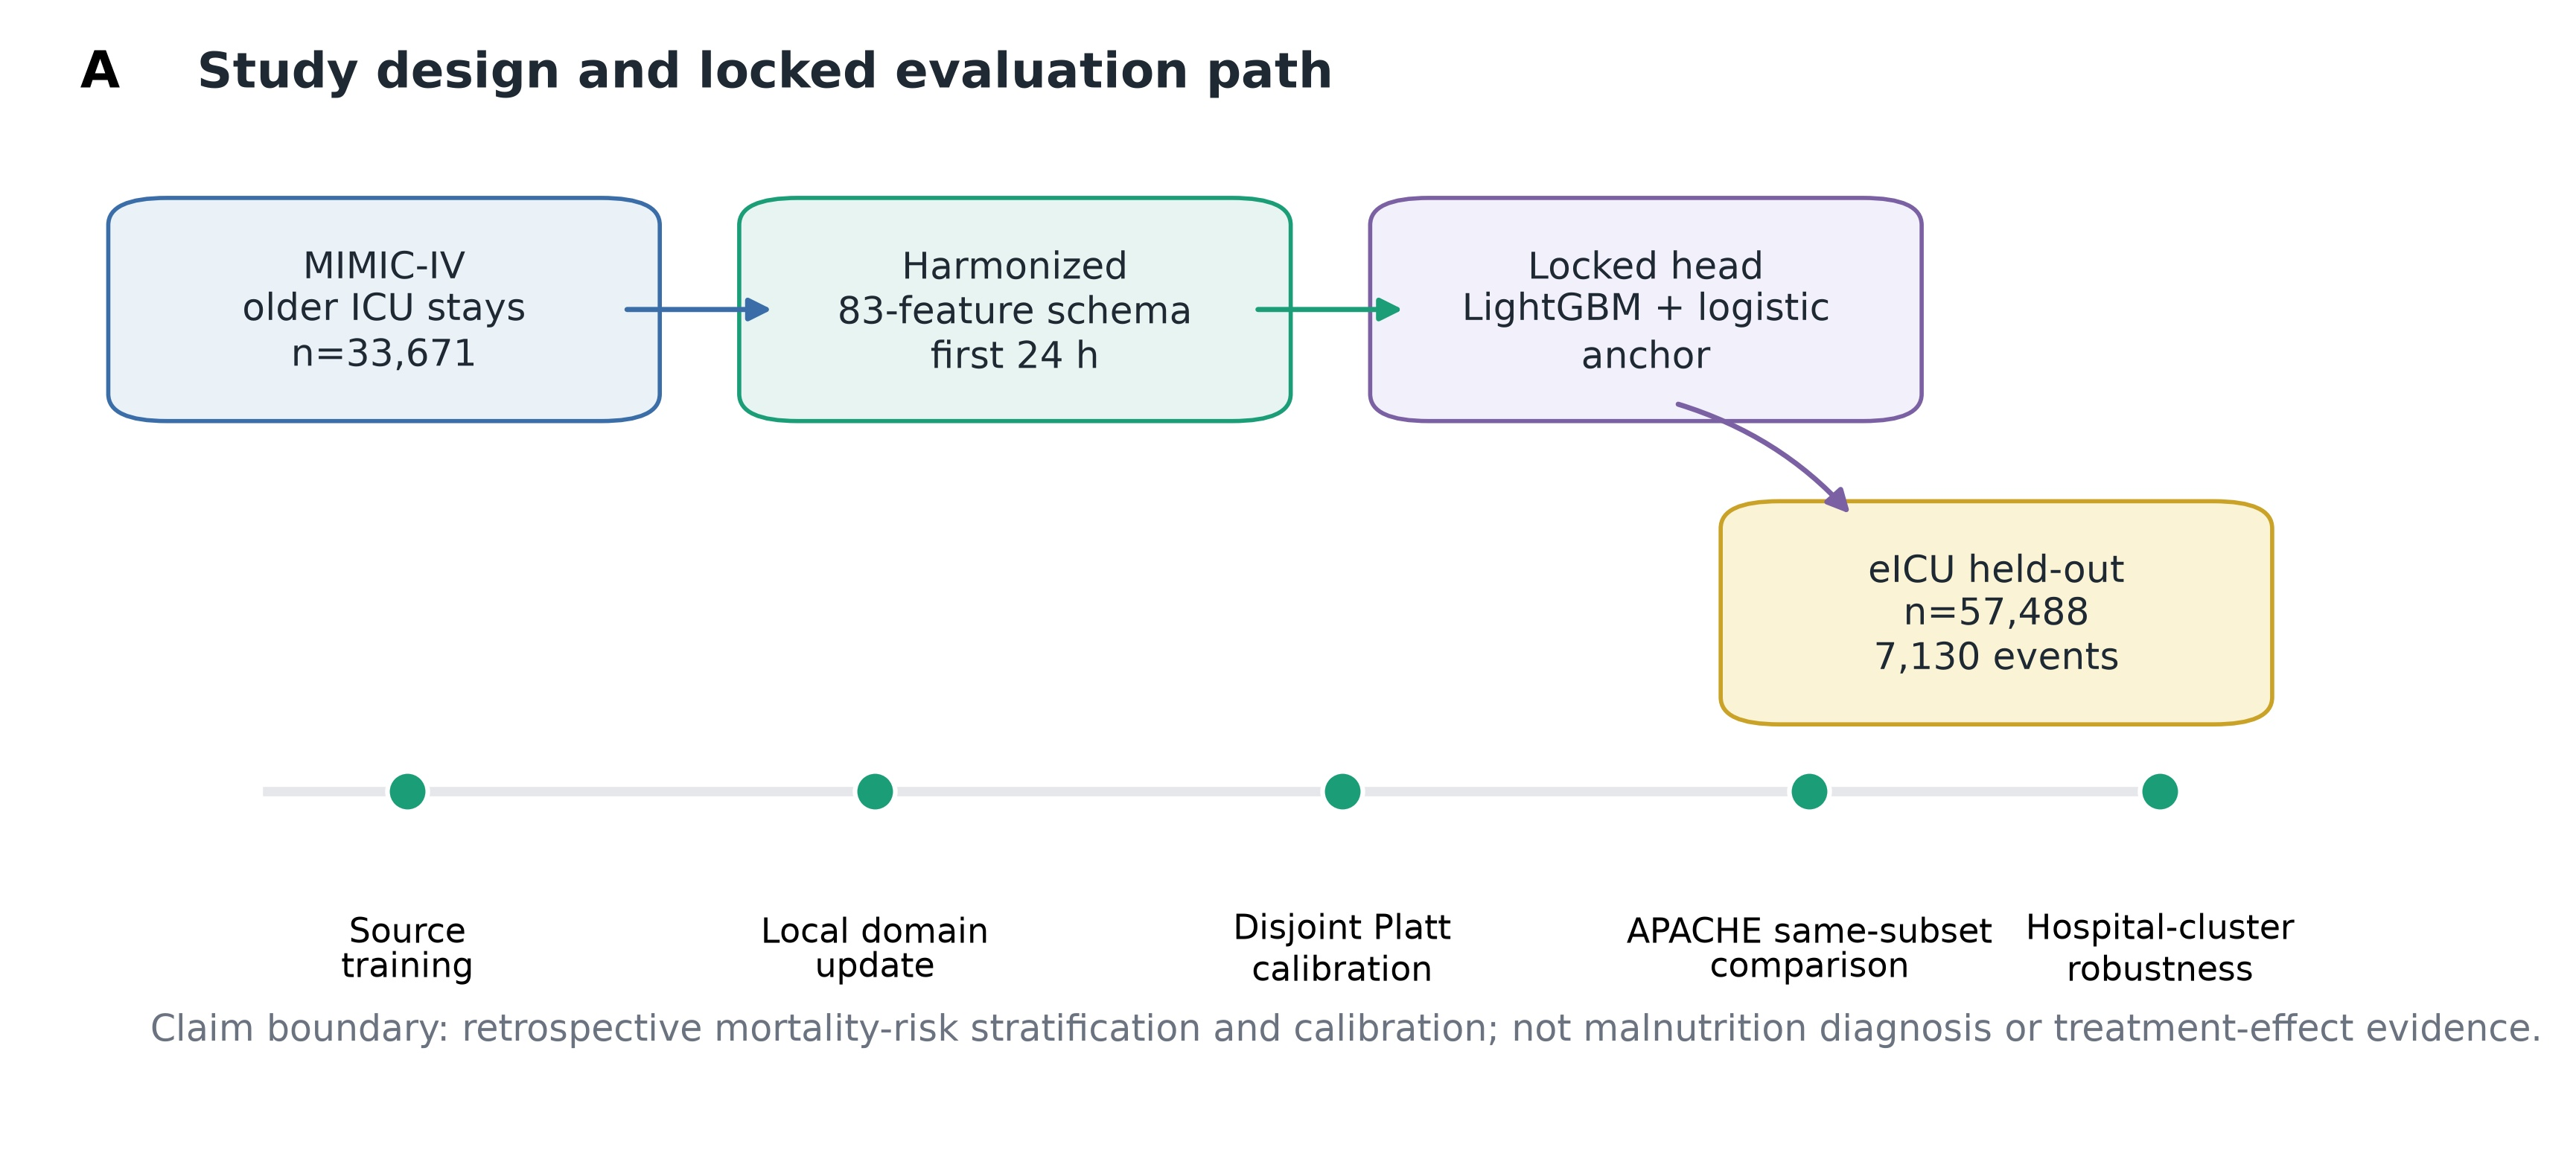
\includegraphics[width=0.95\textwidth]{../../figures/main_fig1_workflow.jpg}
\caption{GERI-NutriRisk-ICU 的开发、特征协调、建模、域更新、再校准和持出评估流程。MIMIC-IV v3.1 作为源域开发队列，eICU-CRD 作为目标域外部验证、局部更新、校准和持出评估队列；APACHE-IV/IVa 预测死亡率仅作为同子集临床对照。}
\label{fig:workflow}
\end{figure}

\section{方法}
\subsection{研究设计与数据来源}
本研究采用回顾性多队列预测模型设计，包括一个源域数据库、一个外部目标域数据库，以及预先设定的目标域局部更新、再校准和持出评估路径。MIMIC-IV v3.1 作为源域数据库，用于特征开发、模型训练和内部测试；eICU-CRD v2.0 作为多中心目标域数据库，用于外部验证、局部更新、校准和持出评估 \citep{PhysioNetMIMICIV31,PhysioNetEICU20,Johnson2023MIMICIV,Pollard2018EICU}。研究问题定义为老年 ICU 患者入科早期的死亡风险分层，重点关注营养脆弱性、代谢紊乱和急性生理严重程度在同一电子病历特征空间中的共同作用。预测时间点限定在 ICU 入科后第一天，早于住院结局判定。

纳入标准为年龄 65 岁及以上 ICU 住院记录。建模单位采用 ICU 住院而非唯一患者，因为营养支持、生命体征、实验室指标、器官支持和出院结局均依附于具体重症住院过程。源域样本记为 $\mathcal{D}_{S}=\{(\mathbf{x}_{i}^{S},y_{i}^{S})\}_{i=1}^{n_{S}}$，目标域样本记为 $\mathcal{D}_{T}=\{(\mathbf{x}_{i}^{T},y_{i}^{T})\}_{i=1}^{n_{T}}$。患者级数据保留在安全服务器，本地仅保存汇总指标、表格、图源数据、代码日志和非识别化结果。

\subsection{队列与结局}
MIMIC-IV 队列包含 33,671 次 ICU 住院，其中 4,659 次发生目标事件；eICU-CRD 队列包含 71,861 次 ICU 住院，其中 8,860 次发生目标事件。表~\ref{tab:cohort} 给出队列概况。主要终点为院内死亡：MIMIC-IV 使用 admissions 表中的 hospital expire flag，eICU-CRD 使用 patient 表中的 hospital discharge status expired 状态。对第 $i$ 次 ICU 住院，二分类结局定义为
\begin{equation}
y_i =
\begin{cases}
1, & \text{出院状态显示住院期间死亡},\\
0, & \text{出院状态未显示住院期间死亡}.
\end{cases}
\label{eq:outcome}
\end{equation}
公式~\ref{eq:outcome} 给出了两个数据库均可审计、可协调的住院不良结局定义。该终点可用于老年 ICU 人群的营养感知风险分层，因为它反映了重症住院期间的严重不良预后；营养不良状态、营养摄入充分性和营养治疗反应则属于不同临床构念。这个边界决定了全文的解释方式：GERI-NutriRisk-ICU 估计的是营养感知特征空间中的死亡风险，而不是对营养疾病状态作出诊断。

\begin{table}[htbp]
\centering
\caption{队列概况。}
\label{tab:cohort}
\begin{tabular}{lrrrrrr}
\toprule
队列 & 住院数 & 事件数 & 事件率 & 机械通气 & 透析 & GCS 中位数\\
\midrule
MIMIC-IV & 33,671 & 4,659 & 0.138 & 10,920 & 409 & 13\\
eICU-CRD & 71,861 & 8,860 & 0.123 & 14,754 & 1,620 & 15\\
\bottomrule
\end{tabular}
\end{table}

\subsection{变量协调与时间泄漏控制}
预测变量限定为 ICU 入科后前 24 小时内产生的记录，或终点判定前已存在的入院基线字段。设 $a_i$ 为第 $i$ 次 ICU 住院的入科时间，$W_i=[a_i,a_i+24\text{ h}]$ 为特征观察窗。对原始临床测量 $z_{ij}(t)$ 和入院基线字段 $\mathbf{b}_{i}$，第 $j$ 个协调特征由预设提取和映射算子生成：
\begin{equation}
x_{ij}=H_j\left(\{z_{ij}(t):t\in W_i\},\mathbf{b}_{i}\right),\quad j=1,\ldots,p,
\label{eq:feature_map}
\end{equation}
其中锁定完整特征模式下 $p=83$。公式~\ref{eq:feature_map} 是时间泄漏控制的核心：特征向量 $\mathbf{x}_{i}$ 可以使用早期时间窗内的测量值和入院背景字段，但不能使用出院状态、住院时长、基线时间窗后的操作记录或任何由结局派生的变量。

最终特征模式包括人口学、BMI、早期肠内/肠外营养支持、白蛋白、血糖、肌酐、尿素氮、钠、胆红素、红细胞压积、白细胞计数、生命体征、乳酸和 PaO$_2$/FiO$_2$ 等血气/灌注指标、凝血/血液学指标、尿量、机械通气、透析、Glasgow 昏迷评分、ICU 类型和入院来源。对临床上具有信息量且可跨数据库映射的缺失指示变量予以保留：
\begin{equation}
m_{ij}=I(x_{ij}\ \text{在}\ W_i\ \text{内未被观测}).
\label{eq:missingness}
\end{equation}
公式~\ref{eq:missingness} 将缺失性视为电子病历观测过程的一部分，而不是单纯的数据清洗问题。在 ICU 数据中，某项指标是否被检测往往与分诊、病情严重程度、临床怀疑和诊疗流程有关，因此可映射的缺失指示变量本身具有预测信息。跨数据库协调要求每个保留特征均具备明确 MIMIC-IV 来源、eICU-CRD 来源、方向一致的临床含义和显式缺失处理。

\subsection{GERI-NutriRisk-ICU 框架}
GERI-NutriRisk-ICU 区分四个功能模块：用于系数级解释的标准化逻辑回归锚定模型、方案化表格学习对照、锁定 LightGBM 性能头，以及用于外部域概率尺度修正的 Platt 再校准层。对所有模型族，未校准风险函数统一写为
\begin{equation}
\hat{p}_i=f_{\theta}(\mathbf{x}_i),\quad 0\leq \hat{p}_i\leq 1,
\label{eq:risk_model}
\end{equation}
公式~\ref{eq:risk_model} 给出了逻辑锚定模型、LightGBM 性能头和各类对照模型共用的风险函数记号，其中 $\hat{p}_i$ 表示公式~\ref{eq:outcome} 所定义住院死亡结局的预测概率。透明锚定模型采用标准化变量和 logistic 链接函数：
\begin{equation}
\hat{p}^{\mathrm{LR}}_i=\sigma\left(\beta_0+\sum_{j=1}^{p}\beta_j\tilde{x}_{ij}\right),\quad
\sigma(u)=\frac{1}{1+\exp(-u)}.
\label{eq:logistic_anchor}
\end{equation}
公式~\ref{eq:logistic_anchor} 用于提供系数层面的可解释锚点和临床方向一致性检查。最终性能头采用 LightGBM，并在相同协调特征表上与 XGBoost、CatBoost、HistGradientBoosting、随机森林、ExtraTrees、多层感知机和 TabNet 进行方案化对照。对照队列覆盖成熟梯度提升模型族 \citep{Chen2016XGBoost,Ke2017LightGBM,Prokhorenkova2018CatBoost} 和神经表格模型 \citep{Arik2021TabNet}。LightGBM 被保留为锁定性能头，是因为没有其他候选模型在保持校准和解释性权衡的同时取得超过 0.015 的实质性 eICU 持出再校准 AUROC 增益。完整模型队列见补充材料。

源域迁移模型仅在 MIMIC-IV 开发集中估计 $\theta$，并将拟合函数不变地应用于 eICU-CRD。域更新性能头则使用 MIMIC-IV 开发数据和预设 eICU 局部更新子集共同拟合。其嵌套训练目标可写为
\begin{equation}
\hat{\theta}_{S+T_u}=
\arg\min_{\theta}
\left[
\frac{1}{|\mathcal{D}_{S}^{\mathrm{dev}}|}
\sum_{i\in \mathcal{D}_{S}^{\mathrm{dev}}}\ell\{y_i,f_{\theta}(\mathbf{x}_i)\}
+
\lambda
\frac{1}{|\mathcal{D}_{T}^{u}|}
\sum_{i\in \mathcal{D}_{T}^{u}}\ell\{y_i,f_{\theta}(\mathbf{x}_i)\}
\right],
\label{eq:domain_update}
\end{equation}
其中 $\ell$ 为二分类预测损失，$\mathcal{D}_{T}^{u}$ 为 eICU 局部更新子集。公式~\ref{eq:domain_update} 明确区分了直接源域迁移和域更新持出验证：目标域标签只用于声明的局部更新子集，最终性能评估在不重叠的 eICU 持出子集中完成。

\subsection{验证与统计分析}
MIMIC-IV 采用固定行索引规则划分开发集和内部测试集。eICU-CRD 进一步划分为不重叠的局部更新、校准和持出评估子集。若 $r_i$ 表示 eICU 固定行索引，则目标域嵌套划分为
\begin{equation}
\mathcal{D}_{T}^{u}=\{i:r_i\bmod 10=0\},\quad
\mathcal{D}_{T}^{c}=\{i:r_i\bmod 10=5\},\quad
\mathcal{D}_{T}^{h}=\{i:r_i\bmod 10\notin\{0,5\}\}.
\label{eq:eicu_split}
\end{equation}
源域迁移分析仅使用 MIMIC-IV 训练模型并评估 eICU，除明确标注的 Platt 再校准外不使用 eICU 标签拟合模型。最终嵌套分析按照公式~\ref{eq:eicu_split} 使用 $\mathcal{D}_{T}^{u}$ 进行局部更新，使用 $\mathcal{D}_{T}^{c}$ 进行校准，使用 $\mathcal{D}_{T}^{h}$ 进行最终持出评估。该划分在记录层面分离局部更新、校准和持出评估；医院层面依赖性则通过站点限制分析和医院聚类 bootstrap 单独检验。

外部域再校准采用 Platt 层，仅在校准子集中拟合，并固定应用于持出集预测：
\begin{equation}
\hat{p}^{\mathrm{cal}}_i=
\sigma\left\{\alpha+\gamma\,\operatorname{logit}(\hat{p}_i)\right\}.
\label{eq:platt}
\end{equation}
公式~\ref{eq:platt} 将风险排序学习与概率尺度修正分离。该设计对于跨数据库预测尤其重要，因为源域模型从 MIMIC-IV 迁移到 eICU-CRD 后可以保留一定风险排序能力，但由于测量频率、编码方式和诊疗流程发生改变，绝对风险概率可能出现明显校准漂移。

模型区分度使用 AUROC 评估，可解释为随机抽取一个事件住院和一个非事件住院时，事件住院预测风险更高的概率：
\begin{equation}
\operatorname{AUROC}=P(\hat{p}_{i:y_i=1}>\hat{p}_{j:y_j=0}).
\label{eq:auroc}
\end{equation}
校准性能使用 Brier score、ECE 和校准曲线评估。Brier score 定义为
\begin{equation}
\operatorname{Brier}=\frac{1}{n}\sum_{i=1}^{n}(y_i-\hat{p}^{\mathrm{cal}}_i)^2,
\label{eq:brier}
\end{equation}
采用 $K=10$ 个分位数风险箱计算的 ECE 定义为
\begin{equation}
\operatorname{ECE}=\sum_{k=1}^{K}\frac{|B_k|}{n}\left|
\frac{1}{|B_k|}\sum_{i\in B_k}y_i-
\frac{1}{|B_k|}\sum_{i\in B_k}\hat{p}^{\mathrm{cal}}_i
\right|.
\label{eq:ece}
\end{equation}
公式~\ref{eq:auroc}、\ref{eq:brier} 和 \ref{eq:ece} 共同报告，是因为具有良好排序能力的模型仍可能在阈值解释和临床风险沟通中出现概率尺度偏移。

APACHE-IV/IVa 预测死亡率仅作为同子集临床对照，不作为 GERI-NutriRisk-ICU 输入。在 APACHE 可用的 eICU 持出子集中，配对性能差值定义为
\begin{equation}
\Delta_{\mathrm{AUC}}=\operatorname{AUROC}(\hat{p}^{\mathrm{GERI}})-\operatorname{AUROC}(\hat{p}^{\mathrm{APACHE}}),\quad
\Delta_{\mathrm{Brier}}=\operatorname{Brier}(\hat{p}^{\mathrm{GERI}})-\operatorname{Brier}(\hat{p}^{\mathrm{APACHE}}).
\label{eq:paired_delta}
\end{equation}
公式~\ref{eq:paired_delta} 保证临床评分对照建立在完全相同的患者记录上。营养变量增量也采用同样的完整模型减缩减模型配对逻辑，其中正向 $\Delta_{\mathrm{AUC}}$ 和负向 $\Delta_{\mathrm{Brier}}$ 支持完整营养感知特征模式。特征域解释性使用 LightGBM gain 和持出 eICU 集上的分组置换重要性；对于特征组 $G$，分组置换导致的 AUROC 下降定义为
\begin{equation}
\Delta_{\mathrm{perm}}(G)=\operatorname{AUROC}(\hat{p})-\operatorname{AUROC}(\hat{p}^{\pi(G)}),
\label{eq:permutation}
\end{equation}
公式~\ref{eq:permutation} 量化特征域被打乱后带来的持出集区分度损失，其中 $\pi(G)$ 表示仅打乱特征组 $G$，其余预测变量保持不变。临床效用通过决策曲线净获益进行概括：
\begin{equation}
\operatorname{NB}(p_t)=\frac{\operatorname{TP}(p_t)}{n}-\frac{\operatorname{FP}(p_t)}{n}\frac{p_t}{1-p_t},
\label{eq:net_benefit}
\end{equation}
公式~\ref{eq:net_benefit} 中 $p_t$ 为预设风险阈值。医院稳健性通过排除 eICU 样本量最大的 10 家医院、限制持出住院数至少 100 或 200 的医院，以及医院聚类 bootstrap 进行评估。所有最终锁定实验均已在远程分析服务器重新运行，服务器端证据清单记录了 v7--v16 结果文件哈希和日志。

\section{结果}

本章按照逐层验证链条展开。首先通过特征族开发和源域迁移识别哪些信息能够跨数据库保留区分能力，随后评估外部再校准、临床效用、亚组行为和模型类别选择。最终结果集中于锁定域更新框架，并在相同 eICU 记录上与 APACHE-IV/IVa 比较，量化营养变量增量，最后检验解释性和医院层面稳健性。

\subsection{特征族消融}
特征族消融构成了结果证据链的第一层：老年 ICU 死亡风险分层需要超越人口学和营养支持记录的多维早期信息。V0 人口学/BMI/营养支持模式在 eICU 外部验证中的 AUROC 为 0.575；加入实验室指标后升至 0.643，继续加入生命体征后升至 0.666。外部区分度的最大提升出现在纳入一般严重程度变量之后，严重程度基线达到 AUROC 0.722，完整早期 GERI-NutriRisk-ICU 模式达到 AUROC 0.727（图~\ref{fig:ablation}，表~\ref{tab:ablation}）。这一轨迹说明，早期 ICU 死亡风险主要由广义生理脆弱性组织起来；营养相关变量更适合作为该脆弱性背景的一部分进入框架，而器官支持、神经状态和急性生理紊乱提供了更强的跨数据库区分信息。

\begin{figure}[htbp]
\centering
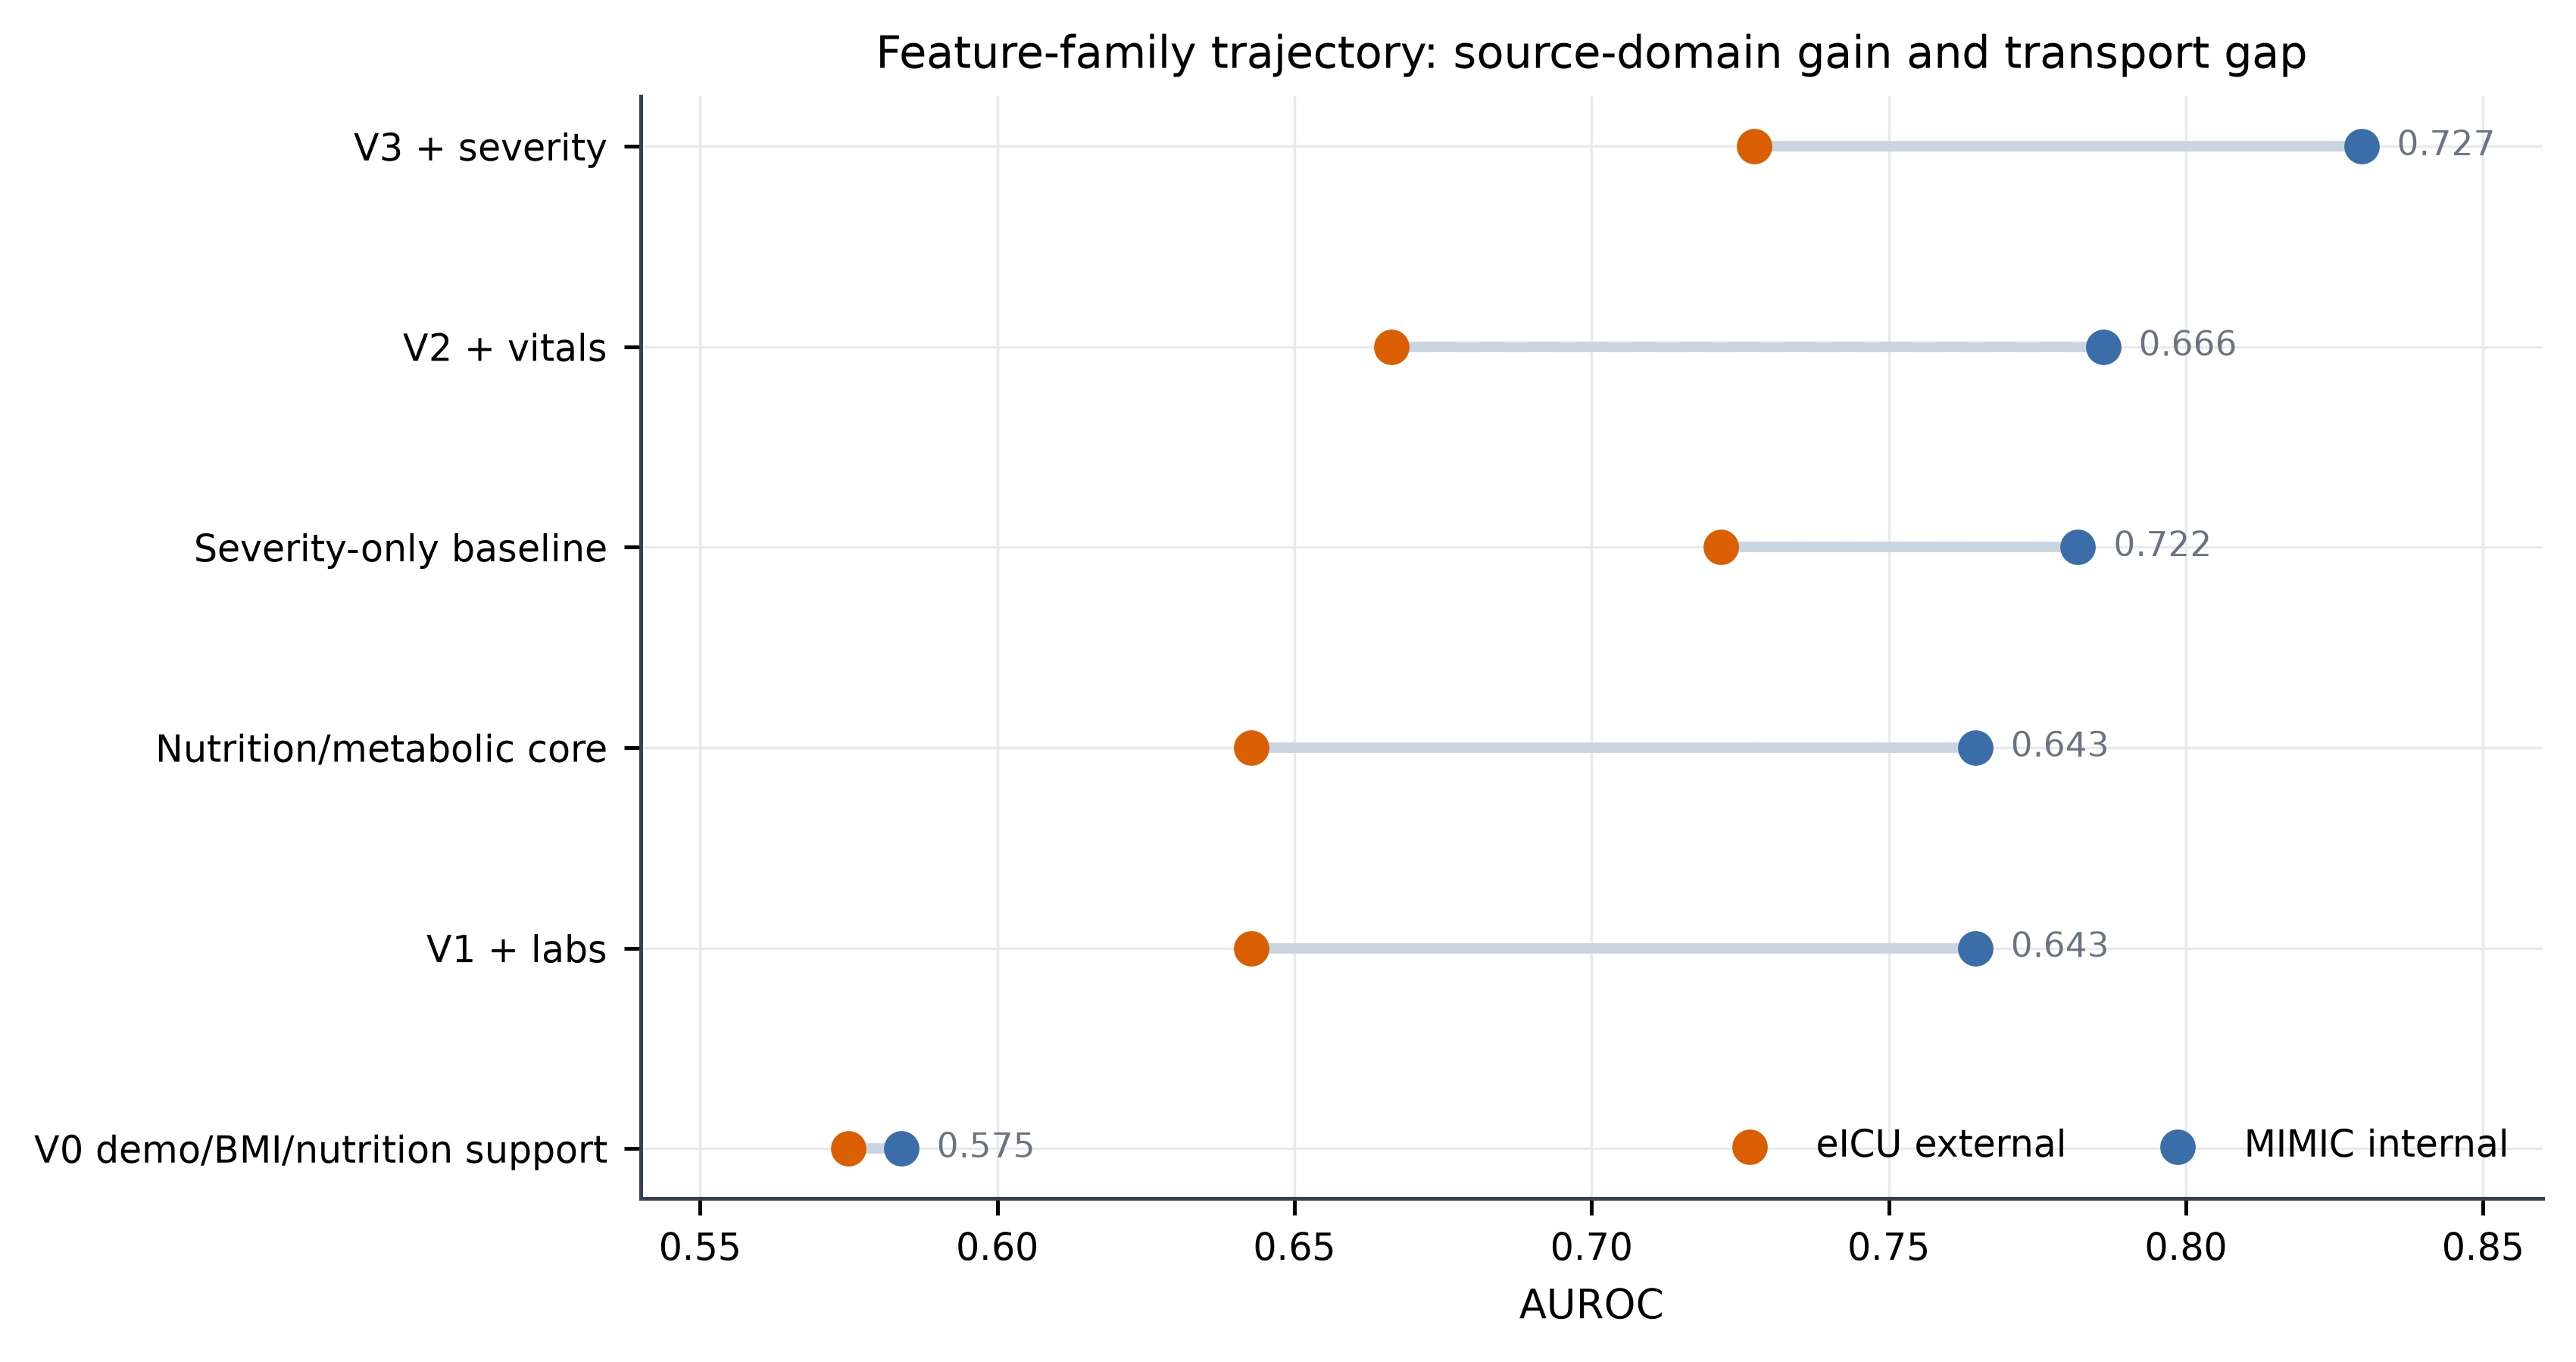
\includegraphics[width=0.85\textwidth]{../../figures/main_fig2_feature_ablation.jpg}
\caption{MIMIC-IV 内部测试和 eICU-CRD 外部验证中的特征族消融。}
\label{fig:ablation}
\end{figure}

\begin{table}[htbp]
\centering
\caption{GERI-NutriRisk-ICU 开发轨迹中的特征族消融结果。粗体表示该列显示结果中的最优值；Brier 越低越好。}
\label{tab:ablation}
\resizebox{\textwidth}{!}{%
\begin{tabular}{lrrrr}
\toprule
特征模式或模型 & MIMIC AUROC & MIMIC Brier & eICU AUROC & eICU Brier\\
\midrule
V0 人口学/BMI/营养支持 & 0.584 & 0.119 & 0.575 & \textbf{0.108}\\
V1 加入实验室指标 & 0.765 & 0.105 & 0.643 & 0.137\\
V2 加入生命体征 & 0.786 & 0.098 & 0.666 & 0.221\\
营养/代谢核心 & 0.765 & 0.105 & 0.643 & 0.137\\
严重程度基线 & 0.782 & 0.098 & 0.722 & 0.119\\
GERI-NutriRisk-ICU & \textbf{0.830} & \textbf{0.090} & \textbf{0.727} & 0.155\\
\bottomrule
\end{tabular}}
\end{table}

预设营养构念敏感性分析进一步区分了营养信息的临床含义和跨库迁移表现。在源域 MIMIC-to-eICU 直接迁移中，完整 V3 模式相对于非营养临床基线的 AUROC 增量为 0.0056（95\% CI 0.0020--0.0090）；同时，去除营养/代谢实验室指标或去除全部营养构念变量的模型在外部队列中具有更好的原始校准指标（表~\ref{tab:nutrition_increment}）。这表明，营养相关测量嵌入了老年重症患者的疾病和脆弱性表型，其变量权重和缺失结构需要经过目标数据库适配后才能形成稳定的外部性能贡献。该结果为后续域更新分析提供了依据，也使域更新成为评价营养变量增量的主要证据层。

\begin{table}[htbp]
\centering
\caption{GERI-NutriRisk-ICU 源域迁移中的营养构念敏感性分析。粗体表示模型行中的最优值；Brier 和 ECE 越低越好。}
\label{tab:nutrition_increment}
\resizebox{\textwidth}{!}{%
\begin{tabular}{lrrr}
\toprule
模型或对比 & eICU AUROC & eICU Brier & eICU ECE\\
\midrule
完整 V3 & 0.727 & 0.155 & 0.180\\
去除营养支持 & 0.726 & 0.151 & 0.170\\
去除营养/代谢实验室指标 & \textbf{0.732} & 0.118 & 0.110\\
去除全部营养构念变量 & 0.729 & \textbf{0.114} & \textbf{0.098}\\
非营养临床基线 & 0.722 & 0.119 & 0.107\\
营养/代谢核心 & 0.643 & 0.137 & 0.137\\
完整 V3 减非营养临床基线 & 0.0056 (0.0020--0.0090) & 0.0364 (0.0355--0.0374) & 0.0726 (0.0716--0.0737)\\
完整 V3 减去除营养/代谢实验室模型 & -0.0050 (-0.0084 至 -0.0020) & 0.0373 (0.0365--0.0383) & 0.0697 (0.0688--0.0707)\\
\bottomrule
\end{tabular}
}
\end{table}

\subsection{主要性能与外部再校准}
在明确源域特征轨迹后，主要性能分析进一步显示：模型在 MIMIC-IV 内部测试中具有较强区分度，跨数据库迁移后出现明显校准漂移。在 MIMIC-IV 内部测试集，GERI-NutriRisk-ICU 的 AUROC 为 0.830（95\% CI 0.815--0.843），Brier score 为 0.090（0.085--0.095），ECE 为 0.015（0.011--0.023）。模型不变地迁移到完整 eICU 队列后，AUROC 降至 0.727（0.722--0.733），Brier score 为 0.155（0.153--0.156），ECE 为 0.180（0.177--0.182）。Platt 再校准基本修正了绝对风险尺度，同时保留风险排序能力：eICU 持出集 AUROC 为 0.728（0.722--0.735），Brier score 改善至 0.099（0.097--0.101），ECE 改善至 0.009（0.008--0.012）（表~\ref{tab:primary}）。图~\ref{fig:calibration} 显示源域迁移后存在校准漂移，同时风险排序仍得到保留；外部 ROC 曲线见中文补充材料图 S1。

\begin{figure}[htbp]
\centering
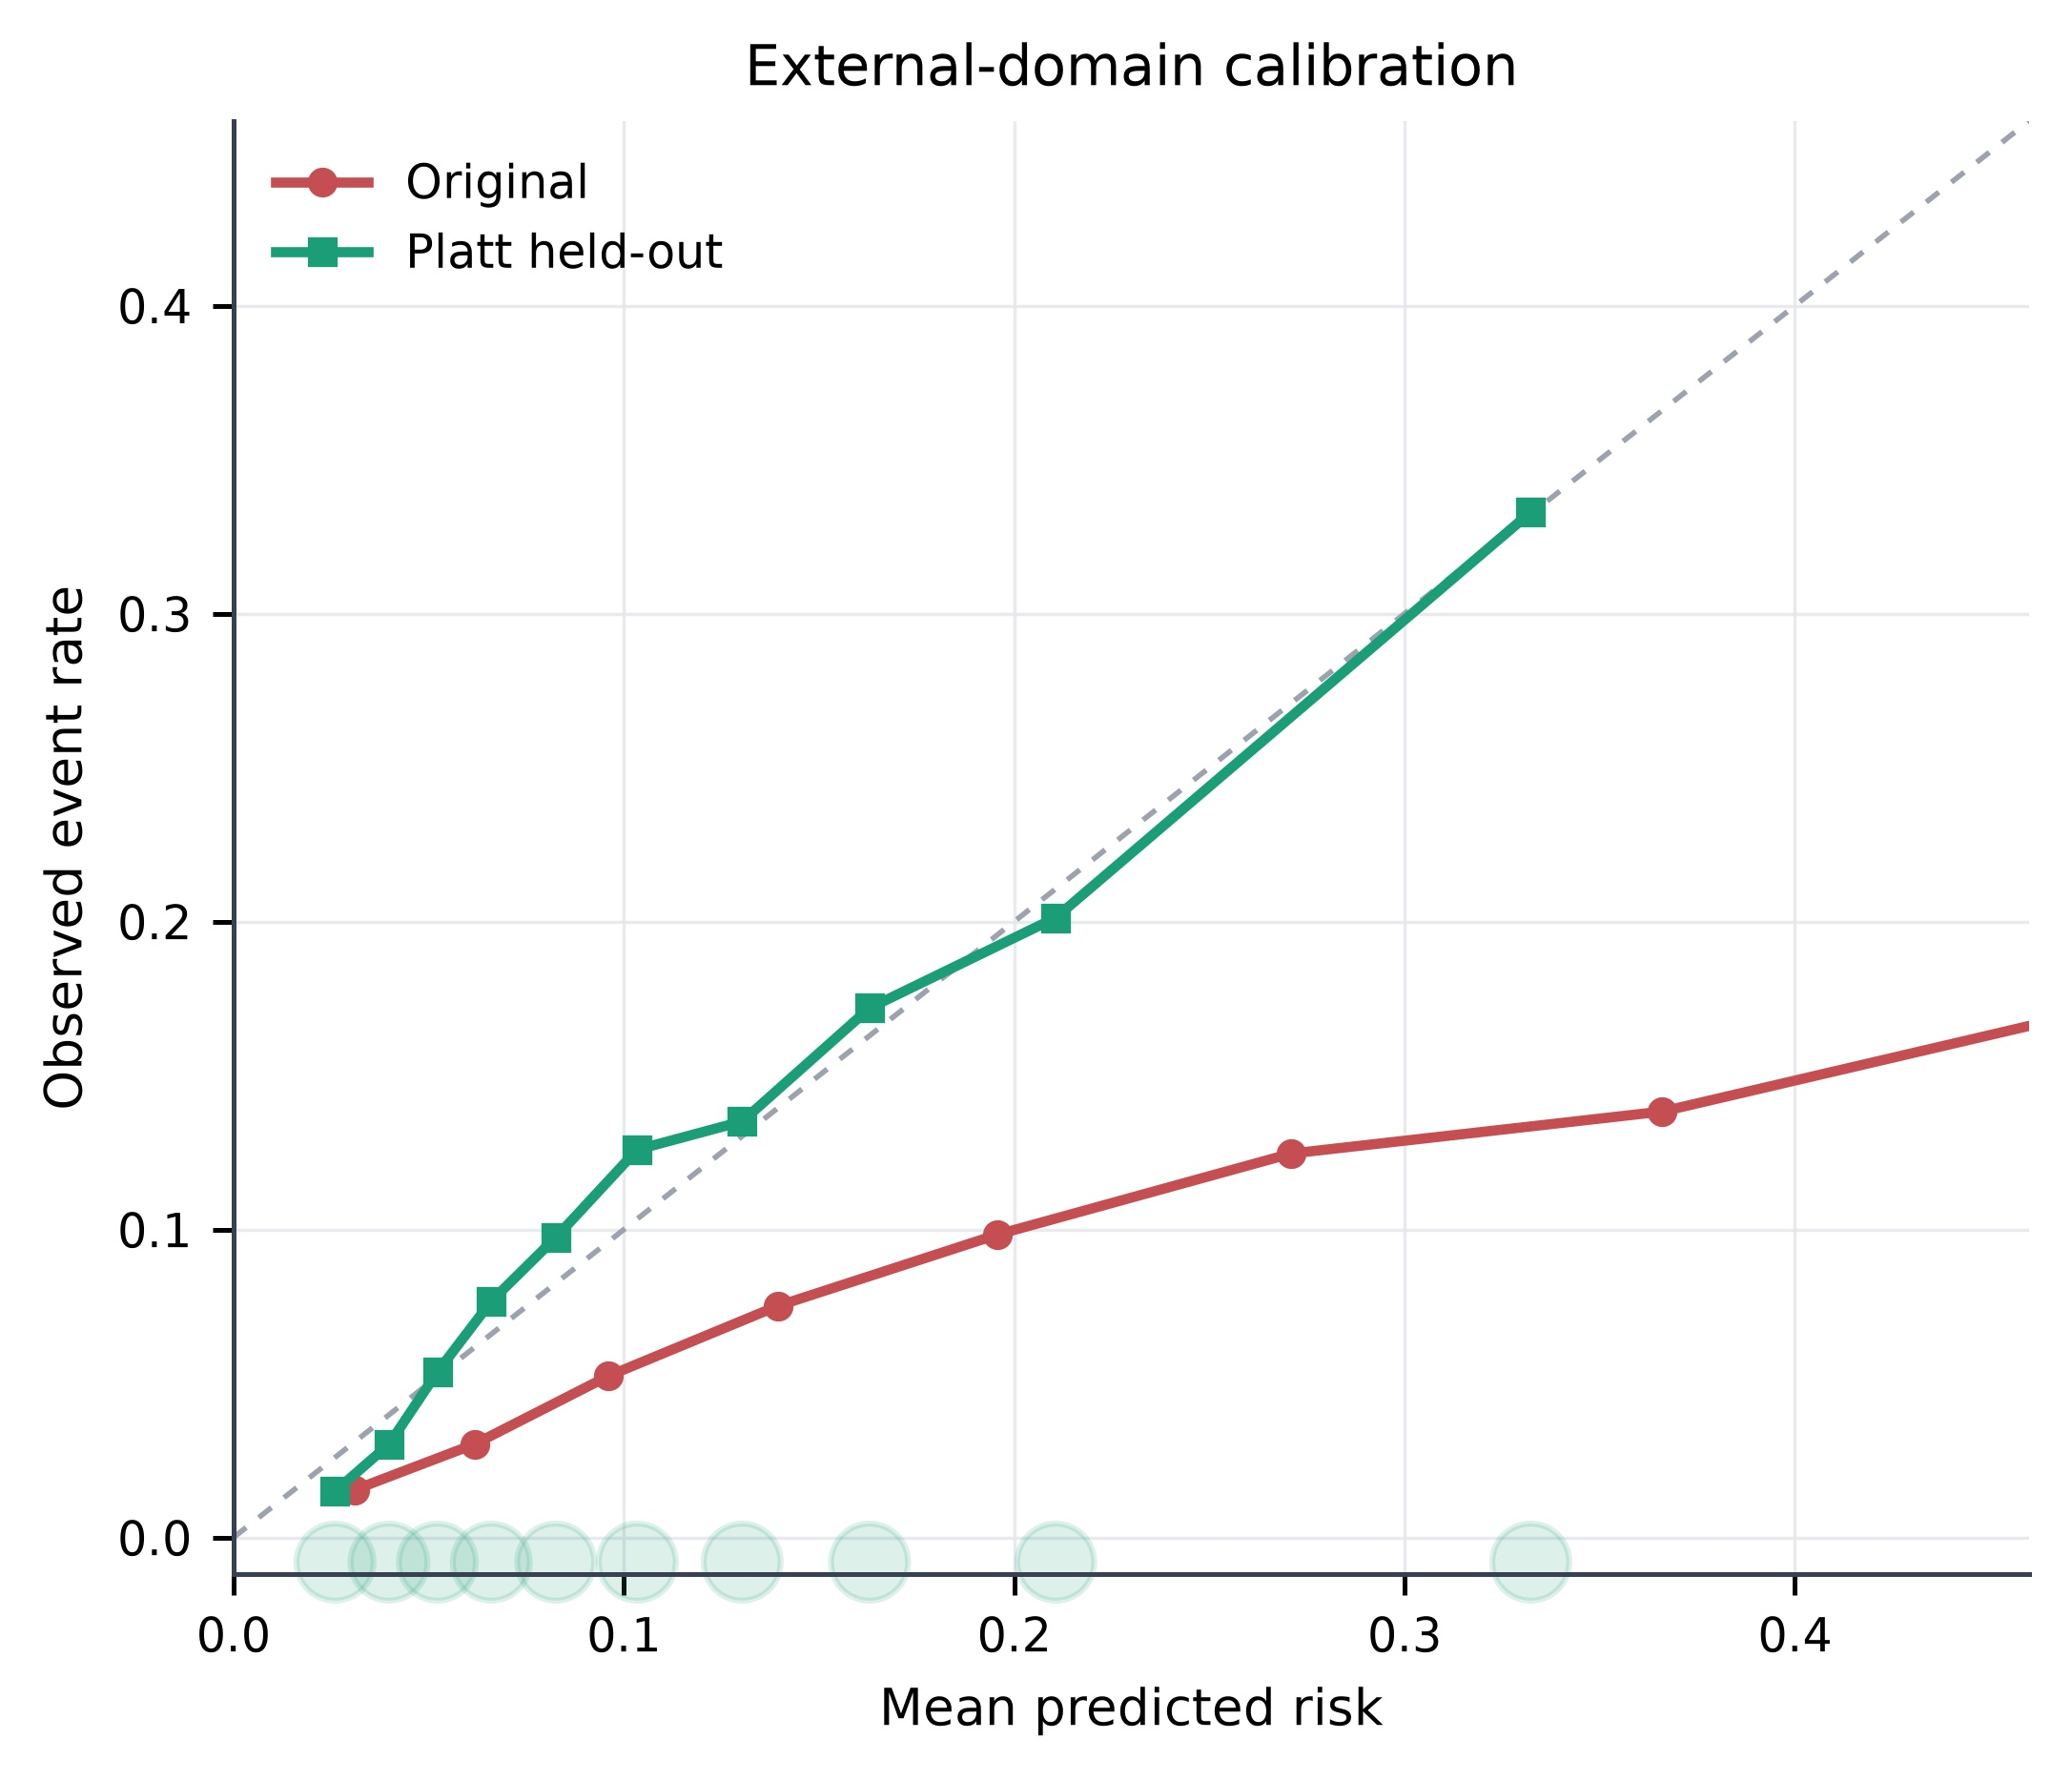
\includegraphics[width=0.68\textwidth]{../../figures/main_fig3_calibration.jpg}
\caption{外部域 Platt 再校准前后的校准曲线。}
\label{fig:calibration}
\end{figure}

\begin{table}[htbp]
\centering
\caption{主要模型性能及 bootstrap 置信区间。}
\label{tab:primary}
\resizebox{\textwidth}{!}{%
\begin{tabular}{lrrlll}
\toprule
评估集 & N & 事件数 & AUROC & Brier & ECE\\
\midrule
MIMIC-IV 内部测试 & 6,735 & 946 & 0.830 (0.815--0.843) & 0.090 (0.085--0.095) & 0.015 (0.011--0.023)\\
eICU 完整外部验证 & 71,861 & 8,860 & 0.727 (0.722--0.733) & 0.155 (0.153--0.156) & 0.180 (0.177--0.182)\\
eICU 持出集再校准 & 57,488 & 7,130 & 0.728 (0.722--0.735) & 0.099 (0.097--0.101) & 0.009 (0.008--0.012)\\
\bottomrule
\end{tabular}
}
\end{table}

\subsection{临床效用、亚组与可解释性}
外部再校准改善绝对风险尺度后，决策曲线将这一变化转化为阈值层面的临床效用证据。源域轨迹在较低到中等风险阈值范围内具有正净获益，再校准后预测概率与观察风险更接近，阈值曲线也更平稳（中文补充材料图 S2）。亚组分析进一步检验了外部行为：模型在不同性别中的 AUROC 接近，在机械通气患者中区分度更高，而在 85 岁及以上患者中较低，提示极高龄患者的死亡风险可能受到更复杂的衰弱负担和结局异质性影响。白蛋白可用者 AUROC 高于白蛋白缺失者（0.785 vs. 0.704），说明更完整的营养/代谢测量可以捕捉额外的疾病和脆弱性结构，而不只是增加单一实验室指标（表~\ref{tab:subgroup}）。透明逻辑锚定模型的标准化系数也具有临床一致性：较低 GCS、较低尿量、较高呼吸频率、较高 BUN、年龄和血糖均对应更高风险方向（中文补充材料图 S3）。这些结果支持模型风险排序的面向临床解释。

\begin{table}[htbp]
\centering
\caption{eICU 外部验证主要亚组表现。}
\label{tab:subgroup}
\begin{tabular}{llrrrr}
\toprule
维度 & 亚组 & N & 事件数 & AUROC & Brier\\
\midrule
性别 & 女性/其他 & 34,780 & 4,330 & 0.723 & 0.163\\
性别 & 男性 & 37,081 & 4,530 & 0.733 & 0.147\\
年龄 & 65--74 & 31,322 & 3,114 & 0.737 & 0.129\\
年龄 & 75--84 & 26,004 & 3,391 & 0.717 & 0.163\\
年龄 & 85+ & 14,535 & 2,355 & 0.702 & 0.196\\
白蛋白 & 缺失 & 49,861 & 5,209 & 0.704 & 0.165\\
白蛋白 & 可用 & 22,000 & 3,651 & 0.785 & 0.133\\
机械通气 & 否 & 57,107 & 4,749 & 0.720 & 0.151\\
机械通气 & 是 & 14,754 & 4,111 & 0.754 & 0.171\\
肠内营养 & 否 & 63,935 & 7,580 & 0.727 & 0.151\\
肠内营养 & 是 & 7,926 & 1,280 & 0.716 & 0.185\\
\bottomrule
\end{tabular}
\end{table}

\subsection{划分稳定性与 SOTA 表格模型对照}
在确认透明逻辑锚定模型具有稳定外部行为后，模型类别对照用于判断是否需要引入非线性性能头。五次固定行索引轮换显示，逻辑锚定模型的外部表现稳定，eICU 原始 AUROC 均值为 0.728（SD 0.002），再校准持出集 Brier score 均值为 0.099（SD $<0.001$；中文补充材料图 S4）。在相同 V3 特征表上，梯度提升模型进一步提高外部区分度，并更有效地捕捉非线性相互作用和跨域特征阈值：LightGBM 完整 eICU 外部 AUROC 为 0.793，XGBoost 为 0.778，CatBoost 为 0.741，逻辑锚定模型为 0.727。轻量神经网络外部迁移较弱，AUROC 为 0.654，提示在该跨数据库表格任务中，特征协调和校准比单纯提高模型灵活性更关键。表~\ref{tab:sota} 汇总初始 SOTA 对照，初始 SOTA 可视化见中文补充材料图 S5。

\begin{table}[htbp]
\centering
\caption{相同 MIMIC-IV 开发集与 eICU-CRD 外部验证集上的 SOTA 表格模型对照。粗体表示该列显示结果中的最优值；Brier 和 ECE 越低越好。}
\label{tab:sota}
\resizebox{\textwidth}{!}{%
\begin{tabular}{lrrrrrr}
\toprule
模型 & MIMIC AUROC & MIMIC Brier & eICU AUROC & eICU Brier & eICU ECE & eICU Platt Brier\\
\midrule
Logistic regression & 0.830 & \textbf{0.090} & 0.727 & \textbf{0.155} & \textbf{0.180} & 0.099\\
XGBoost & 0.880 & 0.136 & 0.778 & 0.297 & 0.392 & 0.092\\
CatBoost & 0.881 & 0.138 & 0.741 & 0.377 & 0.479 & 0.099\\
GERI-NutriRisk-ICU & \textbf{0.882} & 0.124 & \textbf{0.793} & 0.291 & 0.386 & \textbf{0.088}\\
\bottomrule
\end{tabular}
}
\end{table}

\subsection{封顶 SOTA 补充与模型锁定}
扩展后的封顶 SOTA 队列用于检验是否存在足以替换 LightGBM 的实质性模型收益。HistGradientBoosting 在再校准 eICU 持出集中取得数值最高 AUROC（0.794），与 LightGBM 基本持平，但差异仅为 0.00010，且 LightGBM 的再校准 Brier score 更低（0.088 vs. 0.089）。随机森林、ExtraTrees 和多层感知机均低于梯度提升模型的外部区分度；GPU 训练的 TabNet 也未改善跨数据库迁移，eICU AUROC 为 0.636，再校准持出集 Brier score 为 0.108。综合区分度、再校准误差、实现稳定性和可解释性输出后，LightGBM 最适合作为 GERI-NutriRisk-ICU 的锁定性能头。表~\ref{tab:sota_lock} 和表~\ref{tab:tabnet} 汇总封顶对照结果，图~\ref{fig:sota_lock} 展示模型锁定结论。

\begin{table}[htbp]
\centering
\caption{封顶 SOTA 补充与 GERI-NutriRisk-ICU 模型锁定对照。粗体表示该列显示结果中的最优值；Brier 越低越好。}
\label{tab:sota_lock}
\resizebox{\textwidth}{!}{%
\begin{tabular}{lrrrrrr}
\toprule
模型 & MIMIC AUROC & MIMIC Brier & eICU AUROC & eICU Brier & eICU Platt AUROC & eICU Platt Brier\\
\midrule
XGBoost & 0.880 & 0.136 & 0.778 & 0.297 & 0.779 & 0.092\\
随机森林 & 0.867 & 0.148 & 0.757 & 0.228 & 0.757 & 0.097\\
CatBoost & 0.881 & 0.138 & 0.741 & 0.377 & 0.742 & 0.099\\
MLP & 0.872 & \textbf{0.082} & 0.676 & 0.291 & 0.677 & 0.102\\
ExtraTrees & 0.830 & 0.182 & 0.674 & 0.304 & 0.676 & 0.104\\
HistGradientBoosting & 0.880 & 0.136 & \textbf{0.793} & 0.221 & \textbf{0.794} & 0.089\\
Logistic regression & 0.830 & 0.090 & 0.727 & \textbf{0.155} & 0.728 & 0.099\\
GERI-NutriRisk-ICU & \textbf{0.882} & 0.124 & \textbf{0.793} & 0.291 & \textbf{0.794} & \textbf{0.088}\\
\bottomrule
\end{tabular}
}
\end{table}

\begin{table}[htbp]
\centering
\caption{TabNet 神经表格模型与 GERI-NutriRisk-ICU 对照。粗体表示该列显示结果中的最优值；Brier 越低越好。}
\label{tab:tabnet}
\resizebox{\textwidth}{!}{%
\begin{tabular}{lrrrr}
\toprule
模型 & MIMIC AUROC & eICU AUROC & eICU Platt AUROC & eICU Platt Brier\\
\midrule
TabNet & 0.857 & 0.636 & 0.636 & 0.108\\
GERI-NutriRisk-ICU & \textbf{0.882} & \textbf{0.793} & \textbf{0.794} & \textbf{0.088}\\
\bottomrule
\end{tabular}}
\end{table}

\begin{figure}[htbp]
\centering
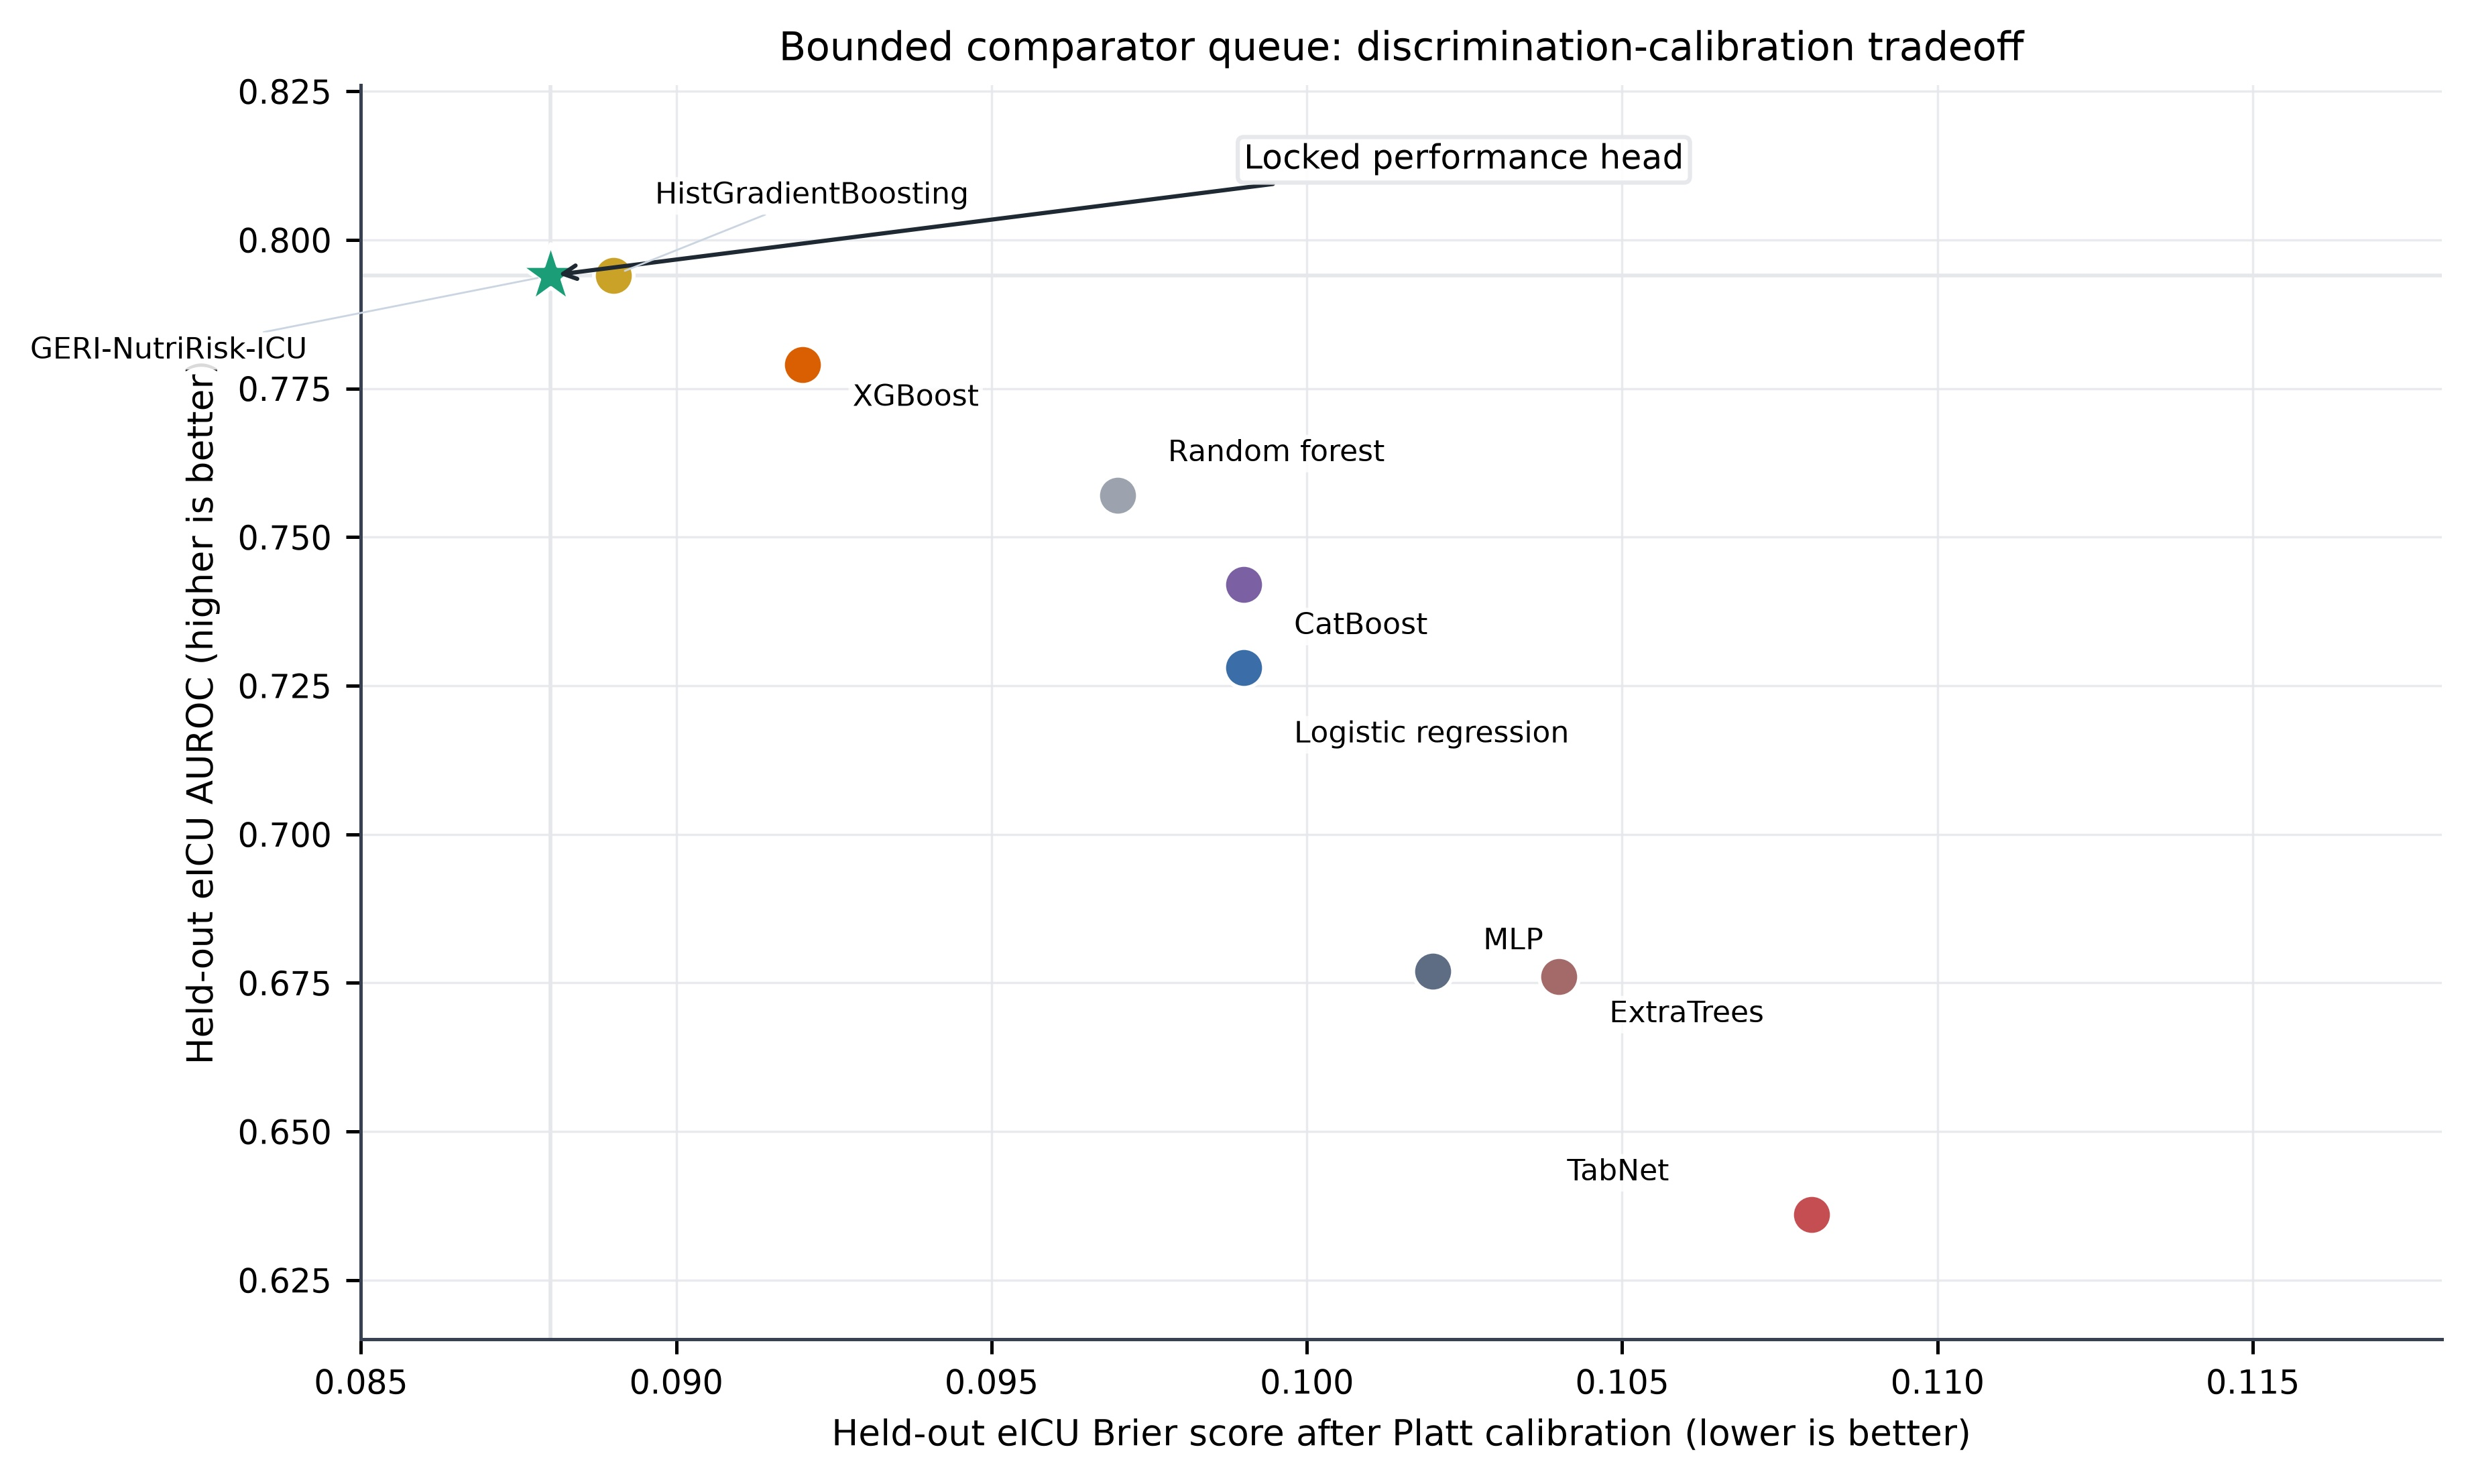
\includegraphics[width=0.95\textwidth]{../../figures/main_fig4_sota_completion_model_lock.jpg}
\caption{封顶 SOTA 补充与模型锁定分析，支持将 LightGBM 保留为最终性能头。}
\label{fig:sota_lock}
\end{figure}


\subsection{锁定域更新性能头}
完成模型锁定后，最终 GERI-NutriRisk-ICU 以 LightGBM 作为性能头，以逻辑回归作为透明解释锚定。协调特征模式进一步扩展至 83 个跨数据库早期变量，并采用嵌套域更新设计：MIMIC-IV 开发数据和预设 eICU 局部更新子集用于模型拟合，不重叠 eICU 子集用于 Platt 校准，其余 eICU 记录用于最终持出评估。在 57,488 次 eICU 持出住院中，锁定模型 AUROC 为 0.872，Brier score 为 0.073，ECE 为 0.004（表~\ref{tab:v14_primary}）。与 83 特征源域加 Platt 模型相比，嵌套域更新将 AUROC 从 0.807 提高至 0.872，并将 Brier score 从 0.085 降至 0.073。由此可见，目标域更新和独立校准是最终框架的核心组成部分。

\begin{table}[htbp]
\centering
\caption{锁定 GERI-NutriRisk-ICU V14 特征集和嵌套域更新模型在 eICU 持出集中的表现。粗体表示该列显示结果中的最优值；Brier 和 ECE 越低越好。}
\label{tab:v14_primary}
\resizebox{\textwidth}{!}{%
\begin{tabular}{llrrr}
\toprule
特征集 & 模型 & AUROC & Brier & ECE\\
\midrule
完整 83 特征模式（源域 + Platt） & GERI-NutriRisk-ICU & 0.807 & 0.085 & 0.014\\
去除全部营养构念变量 & GERI-NutriRisk-ICU & 0.867 & 0.074 & \textbf{0.004}\\
去除显式营养变量 & GERI-NutriRisk-ICU & 0.870 & 0.074 & 0.005\\
去除营养支持指标 & GERI-NutriRisk-ICU & \textbf{0.873} & \textbf{0.073} & \textbf{0.004}\\
去除营养/代谢实验室指标 & GERI-NutriRisk-ICU & 0.866 & 0.074 & \textbf{0.004}\\
完整 83 特征模式（域更新） & GERI-NutriRisk-ICU & 0.872 & \textbf{0.073} & \textbf{0.004}\\
\bottomrule
\end{tabular}
}
\end{table}

\subsection{APACHE-IV/IVa 临床对照}
APACHE-IV/IVa 对照将锁定框架置于成熟 ICU 严重程度评分背景下评价。在同一 eICU 持出评估子集中，39,920 次住院具有 APACHE-IV 和 APACHE-IVa 预测死亡率；这些预测仅作为临床对照，不作为 GERI-NutriRisk-ICU 输入。表~\ref{tab:apache} 显示，锁定模型在同一记录集合中同时优于 APACHE-IV 和 APACHE-IVa 的区分度与 Brier score。与 APACHE-IVa 相比，GERI-NutriRisk-ICU 的 AUROC 为 0.871，APACHE-IVa 为 0.850，配对 AUROC 差值为 0.0209（95\% CI 0.0158--0.0260），Brier score 也更低（0.074 vs. 0.082）。这一结果说明，经过局部更新的营养感知协调框架在 APACHE 式全局严重程度对照之外提供了可测量的风险分辨率，并保持了较好的绝对风险校准。

\begin{table}[htbp]
\centering
\caption{eICU 持出集中 GERI-NutriRisk-ICU 与 APACHE-IV/IVa 的同子集对照。粗体表示同一行中更优的模型或差值；Brier 越低越好。}
\label{tab:apache}
\resizebox{\textwidth}{!}{%
\begin{tabular}{lrrrrr}
\toprule
对照 & 对照 AUROC & 对照 Brier & GERI-NutriRisk-ICU AUROC & GERI-NutriRisk-ICU Brier & AUROC 差值 (95\% CI)\\
\midrule
APACHE-IV & 0.846 & 0.085 & \textbf{0.871} & \textbf{0.074} & \textbf{0.0252} (0.0201--0.0305)\\
APACHE-IVa & 0.850 & 0.082 & \textbf{0.871} & \textbf{0.074} & \textbf{0.0209} (0.0158--0.0260)\\
\bottomrule
\end{tabular}
}
\end{table}

\subsection{锁定模型中的营养增量}
营养相关变量在锁定域更新模型中表现出最清晰的增量贡献。在源域 MIMIC-to-eICU 直接迁移中，多个完整模型减缩减模型的对比为负，说明源域学习到的营养效应对跨数据库编码、测量频率和缺失机制较为敏感。经过局部域更新和不重叠校准后，更广义营养构念以及营养/代谢实验室指标的方向转为正向（表~\ref{tab:v14_nutrition}）。移除全部营养构念变量使 AUROC 降低 0.0049（95\% CI 0.0029--0.0071），Brier score 增加 0.0011；移除营养/代谢实验室指标使 AUROC 降低 0.0059（0.0041--0.0077），Brier score 增加 0.0012。相比之下，早期营养支持指标单独未形成稳定区分增量，提示治疗过程变量的跨库可迁移性弱于代谢测量和脆弱性标志。整体结果支持营养相关变量在完整 ICU 风险框架中提供小幅但可复现的增量价值。

\begin{table}[htbp]
\centering
\caption{eICU 持出集中 GERI-NutriRisk-ICU 的配对营养变量增量。AUROC 差值为正支持完整特征集，Brier 差值为负支持完整特征集；粗体表示最大的有利域更新对比。}
\label{tab:v14_nutrition}
\resizebox{\textwidth}{!}{%
\begin{tabular}{lrrrr}
\toprule
对比 & 源域 AUROC 差值 & 源域 Brier 差值 & 域更新 AUROC 差值 & 域更新 Brier 差值\\
\midrule
完整模型减去去除全部营养构念变量模型 & -0.0184 & 0.0027 & 0.0049 & -0.0011\\
完整模型减去去除显式营养变量模型 & -0.0101 & 0.0021 & 0.0017 & -0.0007\\
完整模型减去去除营养支持指标模型 & -0.0006 & 0.0002 & -0.0005 & -0.0001\\
完整模型减去去除营养/代谢实验室指标模型 & -0.0141 & 0.0024 & \textbf{0.0059} & \textbf{-0.0012}\\
\bottomrule
\end{tabular}
}
\end{table}

\subsection{可解释性与医院聚类稳健性}
V14 锁定模型的解释性分析将性能结果连接到可解释的临床特征域。置换器官支持和神经严重程度造成最大的持出 AUROC 下降（0.0627），其次为生命体征（0.0482）、血气/灌注变量（0.0199）和营养/代谢实验室指标（0.0160）（图~\ref{fig:group_importance}，表~\ref{tab:importance}）。这一排序具有明确的临床含义：模型首先围绕急性器官功能障碍和生理不稳定性组织风险，再由灌注、化学和营养/代谢信息进一步细化风险。主要 gain 特征包括 GCS、钙、BUN、呼吸频率、尿量、乳酸、心率、心脏 ICU 类型、pH 和 BMI（中文补充材料图 S7）。严重程度变量与营养/代谢变量同时进入主要预测特征，说明该框架符合老年 ICU 营养风险分层所需的综合脆弱性建模逻辑。

\begin{figure}[htbp]
\centering
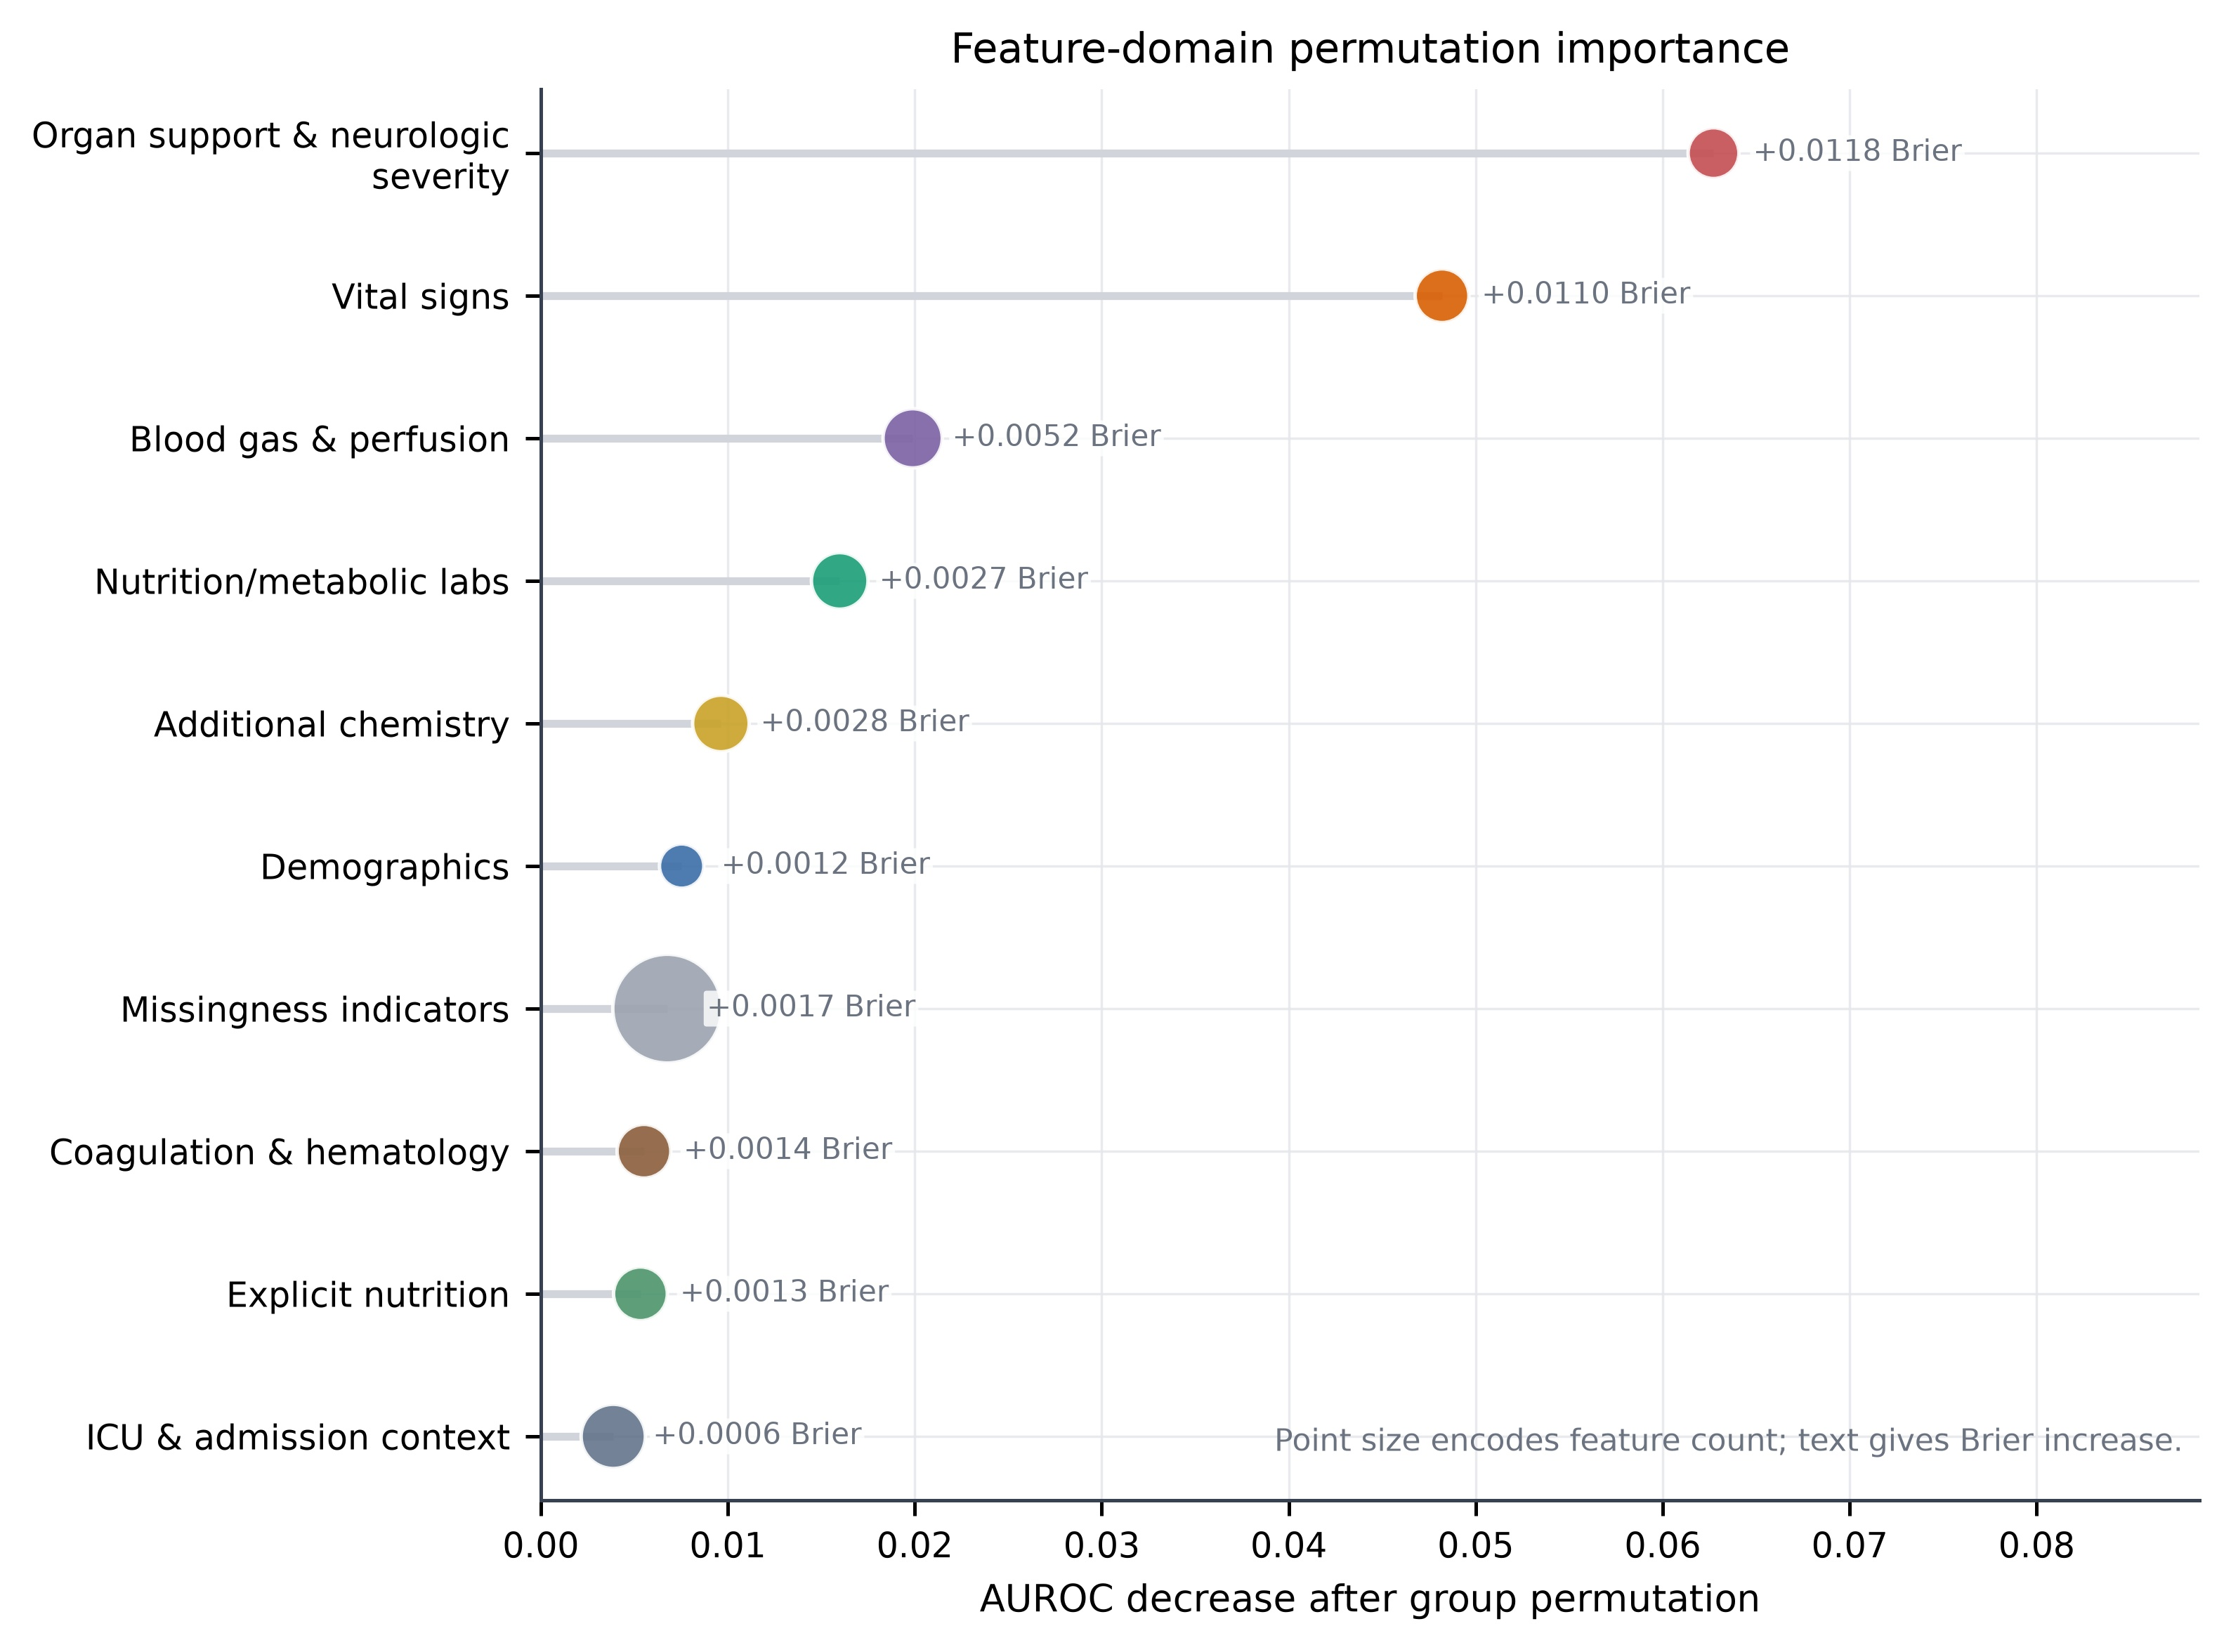
\includegraphics[width=0.72\textwidth]{../../figures/main_fig5_group_permutation_importance.jpg}
\caption{V14 锁定域更新模型的特征域置换重要性。}
\label{fig:group_importance}
\end{figure}

\begin{table}[htbp]
\centering
\caption{分组置换后持出 AUROC 下降幅度最大的特征域。粗体表示最大下降幅度。}
\label{tab:importance}
\begin{tabular}{lrr}
\toprule
特征域 & 特征数 & AUROC 下降\\
\midrule
营养/代谢实验室指标 & 6 & 0.0160\\
额外化学指标 & 6 & 0.0096\\
血气和灌注变量 & 7 & 0.0199\\
生命体征 & 5 & 0.0482\\
器官支持和神经严重程度 & 4 & \textbf{0.0627}\\
\bottomrule
\end{tabular}
\end{table}

医院层面分析检验了 eICU 多中心环境中的性能分布。206 家持出医院中，排除持出样本量最大的 10 家医院后，模型 AUROC 仍为 0.870，Brier score 为 0.072；限制在持出样本量至少 100 或 200 的医院中，AUROC 分别为 0.874 和 0.875（表~\ref{tab:hospital}）。不同医院样本量限制下性能变化很小，说明模型表现分布在不同医院样本量层级中。医院聚类 bootstrap 进一步确认了相对于 APACHE-IVa 的优势，模型减 APACHE-IVa 的 AUROC 差值均值为 0.021，95\% cluster CI 为 0.015--0.028。图~\ref{fig:hospital_auc} 展示医院层面 AUROC 分布，支持锁定框架在多中心 eICU 实践环境中保持区分度的解释。

\begin{table}[htbp]
\centering
\caption{eICU 持出集中 GERI-NutriRisk-ICU 的医院聚类稳健性。粗体表示该列显示结果中的最优值；Brier 越低越好。}
\label{tab:hospital}
\begin{tabular}{lrrrr}
\toprule
分析子集 & N & 事件数 & AUROC & Brier\\
\midrule
全部持出医院 & 57,488 & 7,130 & 0.872 & 0.073\\
排除持出样本量最大 10 家医院 & 44,777 & 5,330 & 0.870 & \textbf{0.072}\\
持出样本量 $\geq$ 100 的医院 & 54,833 & 6,804 & 0.874 & 0.073\\
持出样本量 $\geq$ 200 的医院 & 47,517 & 5,967 & \textbf{0.875} & 0.073\\
\bottomrule
\end{tabular}
\end{table}

\begin{figure}[htbp]
\centering
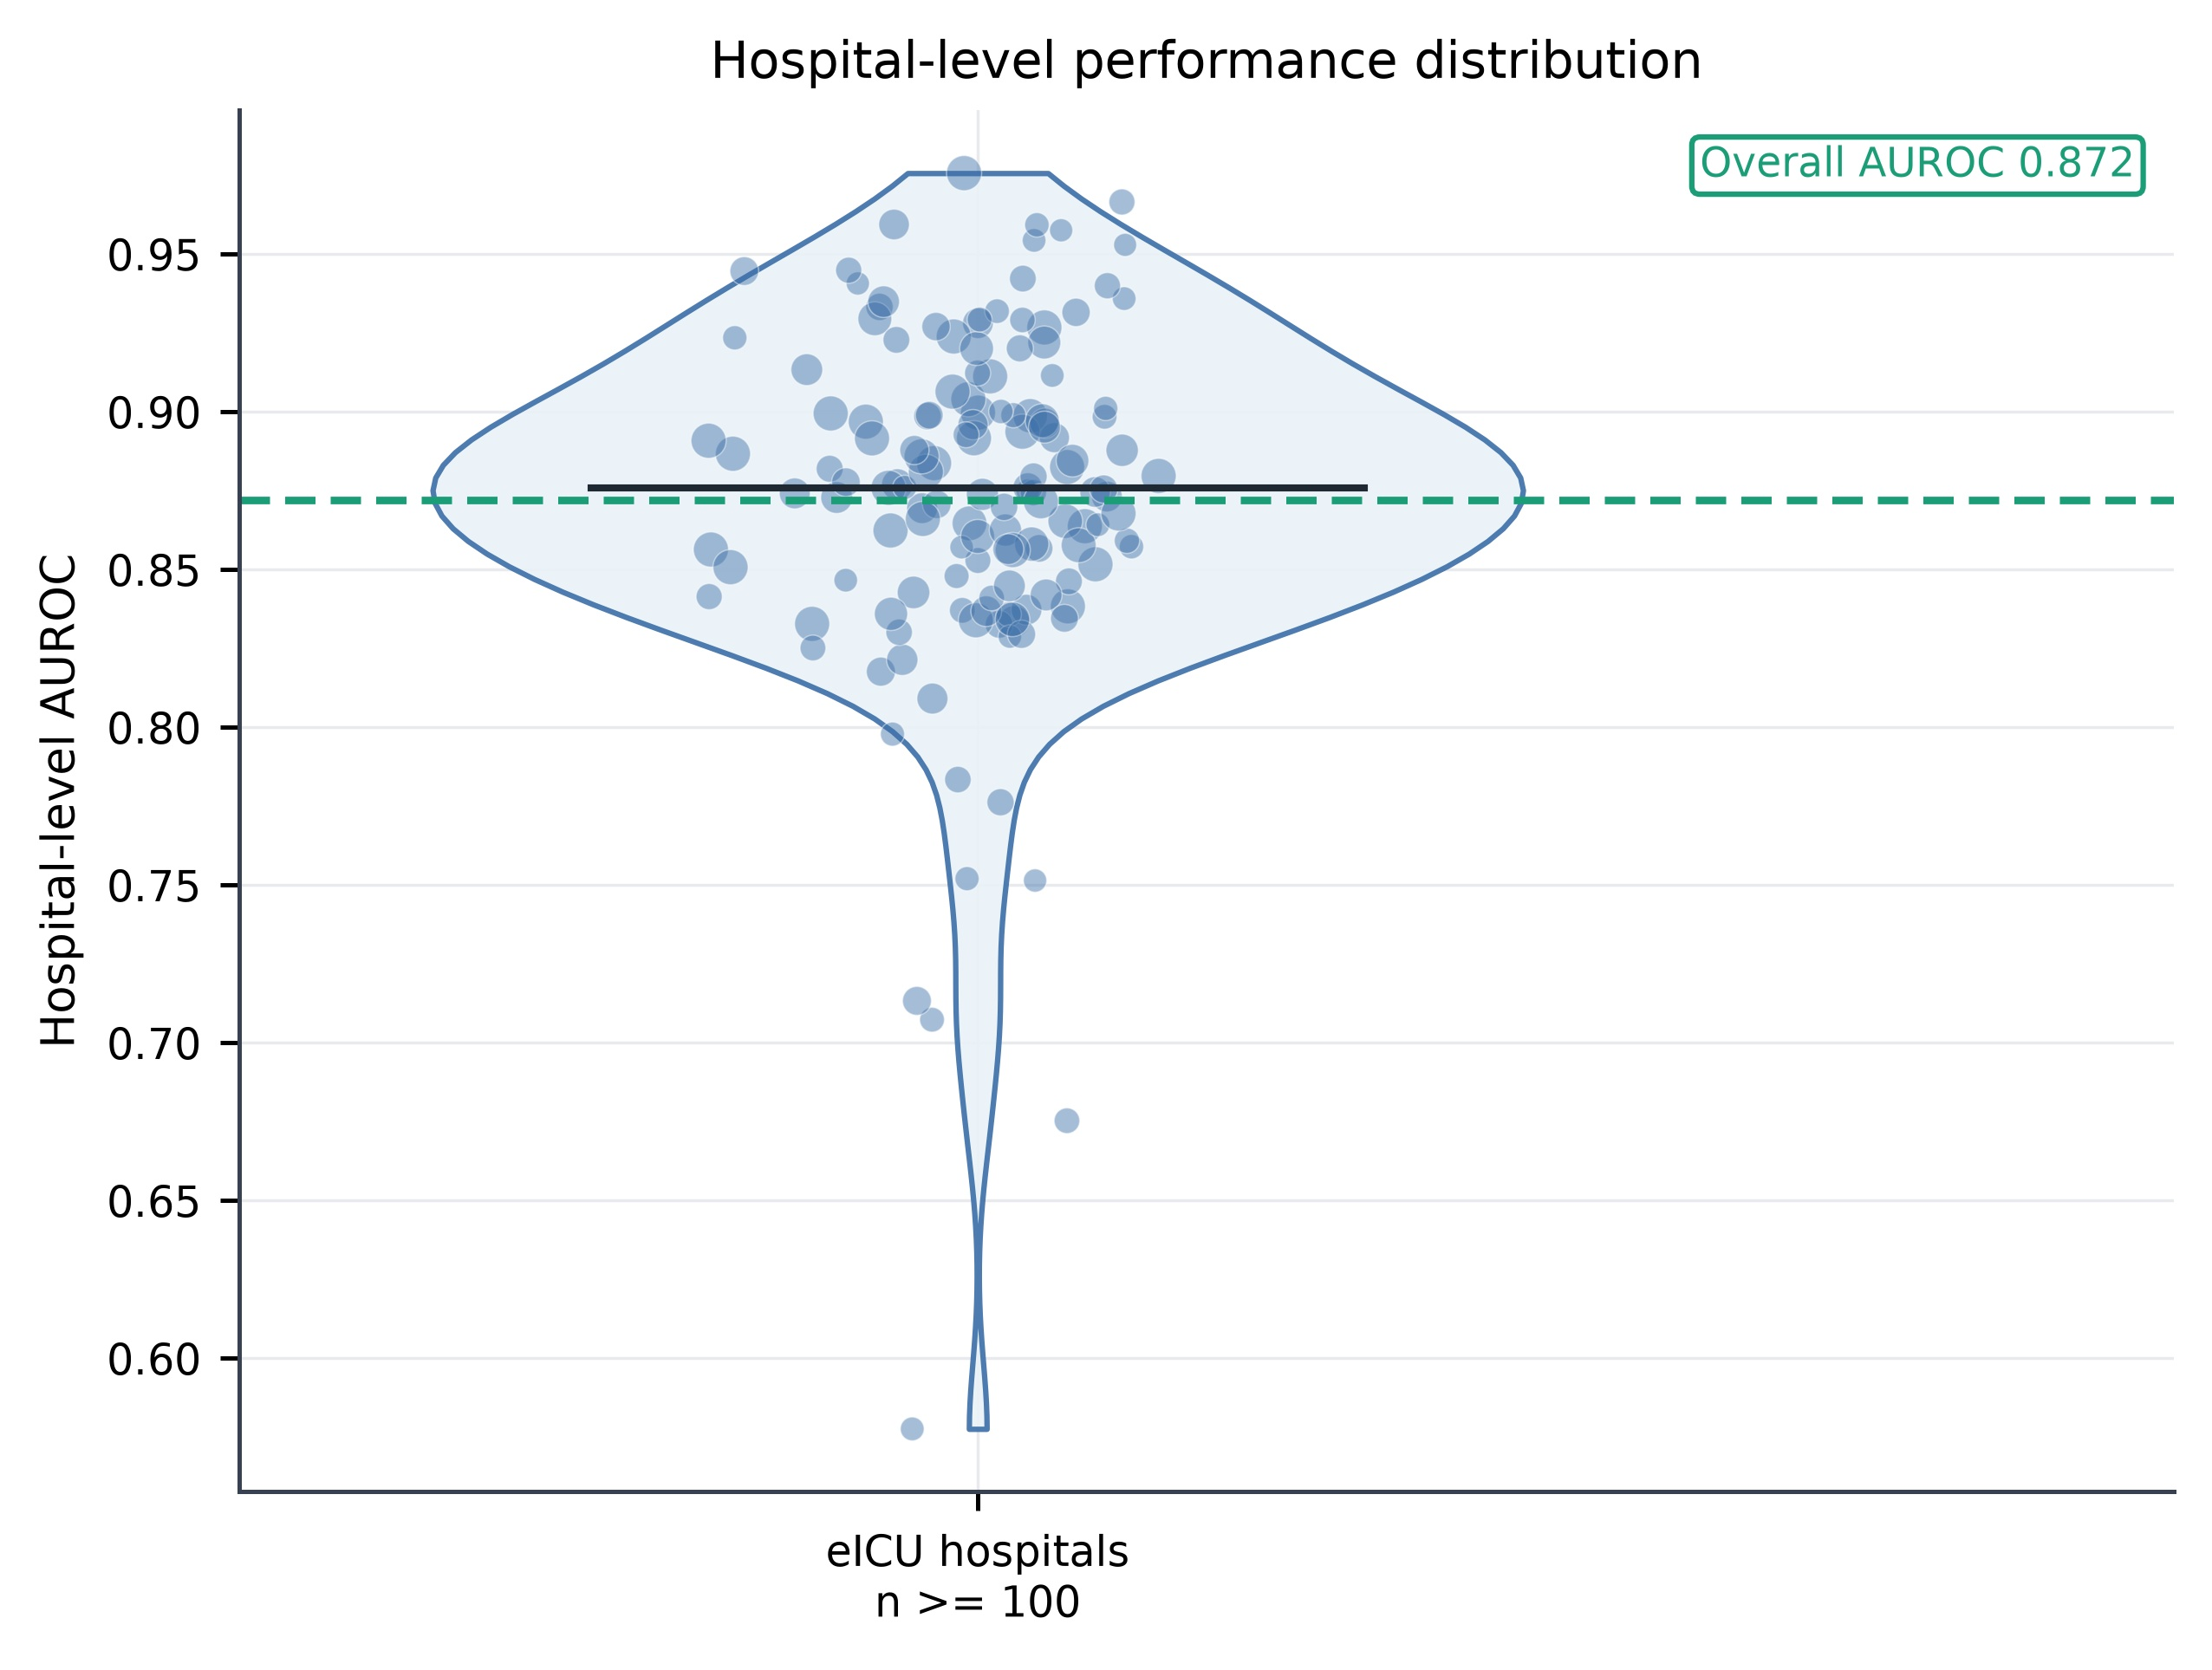
\includegraphics[width=0.70\textwidth]{../../figures/main_fig6_hospital_auc_distribution.jpg}
\caption{持出样本量至少 100 的 eICU 医院层面 AUROC 分布。}
\label{fig:hospital_auc}
\end{figure}

\section{讨论}
本研究开发并外部评估了 GERI-NutriRisk-ICU，一个面向老年 ICU 患者的营养感知死亡风险分层框架。本文的核心结果不是单纯报告某个表格模型取得较高 AUROC，而是证明在协调后的老年 ICU 特征空间中，通过预设目标域更新和不重叠校准，可以形成具有 APACHE 对照、概率校准、可解释性和多中心稳健性的风险分层证据链。对于营养相关重症预测研究而言，这一点尤其关键，因为营养变量与急性严重程度、检测频率、器官支持、医嘱流程和数据库记录方式高度交织。若缺少临床对照和外部验证，营养指标很容易被解释为孤立关联因素。GERI-NutriRisk-ICU 则将营养相关变量置于完整急性严重程度框架内检验，并进一步用 APACHE-IV/IVa、校准指标、决策曲线、特征域归因和医院聚类稳健性共同限定结论。

\subsection{主要结果解释}
APACHE 对照提供了理解本框架增量价值的关键参照。APACHE-IV 和 APACHE-IVa 仍是 ICU 死亡风险预测中的强临床基准，因为它们综合了急性生理、慢性健康状态、诊断和早期治疗背景 \citep{Zimmerman2006ApacheIV}。在本研究中，源域 MIMIC 训练模型经特征扩展后迁移性能有所提高，但在 APACHE 可用 eICU 子集中仍未超过 APACHE-IV/IVa。这一结果建立了必要的基线：当目标数据库在医院构成、工作流、编码习惯和缺失机制上均不同于源数据库时，直接迁移不足以支撑强结论。经过局部域更新和独立校准后，锁定的 GERI-NutriRisk-ICU 性能头在相同 eICU 持出记录上取得 AUROC 0.871，高于 APACHE-IVa 的 0.850，配对 AUROC 差值为 0.0209，同时 Brier score 更低。该增益的绝对幅度属于中等，但其方法学和临床解释价值更强，因为比较对象是同一批患者上的成熟严重程度标准，而不是弱统计基线。

这一结果也明确了框架的使用定位。GERI-NutriRisk-ICU 应被理解为可复现、可局部更新且可校准的老年 ICU 风险分层框架，而不是一个可以在任意医院无修改固定部署的源域评分。模型开发、局部更新、校准和持出评估之间的分离符合当前预测模型研究规范；这些规范强调外部验证、模型更新和最终评估必须被清楚区分 \citep{Collins2024EvalPart1,Riley2024EvalPart2,Collins2024TRIPODAI}。在该设计中，不重叠校准集避免了同一批记录同时用于概率修正和最终评估。最终 eICU 持出集中较低的期望校准误差说明，模型不仅能够排序患者风险，也能输出与观察结局频率更一致的概率估计。

\subsection{营养相关信号的含义}
营养结果进一步限定了本文对营养信息的解释方式。重症营养指南强调早期识别营养脆弱性，但常规电子病历中的结构化变量通常无法单独区分营养不良、摄入充分性或营养治疗反应 \citep{Singer2023ESPENPractical,Compher2022ASPEN,Compher2025GLIMCriticalIllness}。本文消融结果与这一临床现实一致。单独去除营养支持指标没有降低区分度，说明喂养途径记录和早期支持决策本身并不足以作为稳定预测标志。相反，去除更广义的营养构念变量和去除营养/代谢实验室指标分别使域更新模型 AUROC 下降 0.0049 和 0.0059，完整模型同时具有更好的 Brier score。这些配对比较表明，营养相关信息在与器官支持、生命体征、血气/灌注变量和入院背景共同建模时，能够提供可测量的增量价值。

解释性分析支持同一结论。分组置换显示，器官支持和神经严重程度造成最大的 AUROC 损失，其次为生命体征和血气/灌注变量，说明模型的主要风险结构仍由急性重症状态主导。与此同时，营养/代谢实验室指标的重要性高于部分背景变量和缺失指示变量，单变量 gain 排序中也出现了 BUN 和 BMI。由此可见，本文并不主张某个单一营养干预可以改变死亡风险；更准确的结论是，营养和代谢变量能够在主要严重程度信号之外，帮助识别老年 ICU 患者之间的残余风险异质性。这一解释符合老年重症医学的病理生理逻辑，即营养储备、分解代谢、肾脏和代谢应激、衰弱以及急性器官功能障碍共同决定短期脆弱性。

\subsection{外部有效性、稳健性和临床效用}
eICU-CRD 的多中心结构增强了外部评估的实际意义，因为该数据库包含多个医院、不同病例组合和异质化记录流程 \citep{Pollard2018EICU}。单一总体 AUROC 可能掩盖模型收益集中在少数大样本医院的情况。本文医院层面分析针对这一问题进行了检验：排除样本量最大的 10 家医院后，模型 AUROC 仍保持在 0.870；限制在持出样本量至少 100 或 200 的医院时，AUROC 分别为 0.874 和 0.875。医院聚类 bootstrap 也维持了相对于 APACHE-IVa 的正向 AUROC 差值。上述结果说明，模型相对于 APACHE-IVa 的优势并非完全由高样本量医院驱动，而是在不同医院样本量层级中均能保留。

临床效用不能只由 AUROC 判断。用于营养感知监测的风险分层工具需要同时具备高风险识别能力、概率校准和可操作阈值。本文决策曲线显示，在临床上可能使用的阈值范围内，GERI-NutriRisk-ICU 具有净获益优势；校准结果则显示局部域更新和 Platt 再校准改善了概率对齐。该性质具有实践意义，因为营养评估和营养支持升级高度依赖工作流：过度自信的模型会增加不必要会诊和干预，校准不足的模型则可能漏识别诊断和器官支持变量尚未完全刻画的脆弱老年患者。因此，GERI-NutriRisk-ICU 更适合作为前瞻性风险监测、营养评估优先级排序和老年 ICU 高风险亚组审计的决策支持层。

\subsection{局限性与未来工作}
本研究的结论需要在以下边界内解释。第一，本研究为回顾性分析，受数据库记录方式、测量频率、编码习惯和缺失机制影响。MIMIC-IV 与 eICU-CRD 间的特征协调降低了该问题，但不能使两个数据库在临床流程和数据生成机制上完全一致。第二，主要结局为院内死亡。该终点可审计且具有明确临床意义，但不是营养不良状态、营养摄入充分性、肌肉量、喂养耐受性、功能恢复或营养干预反应的直接测量。第三，优于 APACHE-IV/IVa 的结果适用于嵌套域更新并完成校准后的框架，而不适用于源域 MIMIC-to-eICU 直接迁移模型。若在新机构实施，应先开展本地数据审计、变量映射核查、再校准和前瞻性静默运行评估。

第四，营养相关变量来自常规结构化电子病历，主要反映体型、代谢实验室指标、部分治疗过程和缺失模式，并不包含详细热量和蛋白供给、营养师评估、间接测热、体成分影像或纵向营养轨迹。第五，封顶模型队列降低了事后模型搜索风险，并纳入了传统机器学习和神经表格模型对照，但没有穷尽所有 tabular foundation model、特征工程变体或超参数空间。最后，医院聚类稳健性增强了多中心外部有效性，但不能替代前瞻性实施验证。后续研究应在真实临床工作流中评估 GERI-NutriRisk-ICU，检验校准风险分层能否改善营养评估优先级排序，并进一步观察营养感知监测对流程指标和患者中心结局的影响。

\section{结论}
GERI-NutriRisk-ICU 提供了一个可复现的老年 ICU 早期死亡风险分层框架，具有外部验证、局部更新、概率校准、APACHE 对照和营养感知解释等特征。基于协调后的 MIMIC-IV 和 eICU-CRD 队列，锁定域更新模型在相同 eICU 持出记录上优于 APACHE-IV/IVa，并在不同医院样本量层级中保持稳定；营养/代谢变量则在完整严重程度模型中提供小幅但可复现的增量预测价值。上述结果支持将 GERI-NutriRisk-ICU 作为老年重症营养感知风险监测工具进一步开展前瞻性评价。

\section*{数据可用性}
本研究分析的患者级数据可由完成相应培训和数据使用协议的认证研究者通过 PhysioNet 获取：MIMIC-IV v3.1，\url{https://physionet.org/content/mimiciv/3.1/} 和 \url{https://doi.org/10.13026/kpb9-mt58}；eICU Collaborative Research Database v2.0，\url{https://physionet.org/content/eicu-crd/2.0/} 和 \url{https://doi.org/10.13026/C2WM1R}。作者不能重新分发患者级记录。汇总结果表、图源数据和非识别化可复现材料可在公开代码仓库获取：\url{https://github.com/Hajimi-Sudo/geri-nutririsk-icu}。

\section*{代码可用性}
分析脚本、稿件图表导出脚本、汇总结果表和可复现性清单可在公开 GitHub 仓库获取：\url{https://github.com/Hajimi-Sudo/geri-nutririsk-icu}。该仓库不包含患者级 MIMIC-IV 或 eICU-CRD 记录、派生患者级特征表或任何需要数据使用协议保护的数据库文件。

\section*{伦理声明}
本研究使用通过 PhysioNet 获取的去标识化重症数据库进行二次分析。作者在完成相应资质认证和数据使用协议后访问并分析数据。研究过程不涉及直接患者接触或再识别。

\section*{作者贡献}
ZJ：概念化、方法学、软件、正式分析、初稿撰写。HS：方法学、验证、数据整理、审阅与修改。YZ：软件、基准整理、可视化、可复现性审计。SW：监督、资源、项目管理、审阅与修改。

\section*{经费支持}
作者声明，本研究、论文写作及发表未获得任何财务支持。

\section*{利益冲突}
作者声明不存在可被解释为潜在利益冲突的商业或财务关系。

\bibliographystyle{Frontiers-Vancouver}
\bibliography{references}

\end{document}
